% This is samplepaper.tex, a sample chapter demonstrating the
% LLNCS macro package for Springer Computer Science proceedings;
% Version 2.21 of 2022/01/12
%


% Camera-ready submissions: All accepted papers must follow the below guidelines to submit your camera-ready papers –

% Your paper should contain your full authors names, full affiliation and ORCID ID (if available). Your submission should contain source files (e.g., latex files or word document). Please read the "Instructions for proceedings authors.pdf" carefully and make sure that you follow these instructions. The link is provided here: (opens in a new window)Instructions for proceedings authors.
% You should print, sign, and scan the "Licence to Publish Proceedings Papers". The license will be provided upon notification of acceptance. 
% Short papers: Authors are invited to submit short papers of length up to 3 pages excluding references (1 column – the LNCS template) showing proof-of-concept research contributions under the topics of the conference. All submissions will be peer-reviewed and the accepted abstracts will be published in Frontiers in Medical Technology as an ebook. Please use the template provided below.

% The word and character limits per short paper are as follows:
% -Title: 500 characters
% -Text: 1,000 words
% -Figures: 2
% -No Supplementary Material

% MIUA continues to foster fairness, diversity, and inclusion within its community. Submissions from typically underrepresented groups are particularly encouraged.

% https://www.ucd.ie/medicine/miua2026/calls/callforpapers/

% Reviewer #1
% Questions
% 1. Please provide major strengths of the paper.
% The paper presents a fetal ultrasound synthesis framework and shows that models trained on the proposed dataset achieve better performance than those trained on datasets used in previous work.

% 2. Please provide any major weaknesses of the paper.
% Although this is a short paper, the technical contribution appears weak. The proposed method is based on the existing EDM2 latent diffusion model, and the paper provides very limited implementation details, with no description of the training configuration beyond the loss function.


% 3. Overall evaluation of the paper.
% Accept


% 6. Constructive feedback to authors for improving the paper. (optional)
% It would be useful to include results from different network architectures trained on the same dataset with identical training configurations. The current version does not clearly demonstrate whether the observed performance is attributable to the EDM2 architecture or to the dataset used for training.

% KEY DATES
% Full Paper Submission: Thursday 2nd April 2026 (01:00 Pacific Time (PT))
% Notification of Acceptance: Friday 5th June 2026 
% Camera Ready Deadline: Friday 12th June 2026
% Early Registration: Friday 12th June 2026





\documentclass[runningheads]{llncs}
%
\usepackage[T1]{fontenc}
% T1 fonts will be used to generate the final print and online PDFs,
% so please use T1 fonts in your manuscript whenever possible.
% Other font encondings may result in incorrect characters.
%
\usepackage{booktabs} 
\usepackage{graphicx}
\usepackage{multirow}
\usepackage{orcidlink}
% Used for displaying a sample figure. If possible, figure files should
% be included in EPS format.
%
% If you use the hyperref package, please uncomment the following two lines
% to display URLs in blue roman font according to Springer's eBook style:
%\usepackage{color}
%\renewcommand\UrlFont{\color{blue}\rmfamily}
%\urlstyle{rm}

\vspace{-10mm}

\begin{document}
\title{
A Foundational EDM2-Based Generative Model for High-Resolution Synthetic Fetal Ultrasound Imaging from Open Datasets
}
%
%\titlerunning{Abbreviated paper title}
% If the paper title is too long for the running head, you can set
% an abbreviated paper title here
%

%\author{Anonymous Author(s)}

%\authorrunning{Anonymous Author(s)}
% First names are abbreviated in the running head.
% If there are more than two authors, 'et al.' is used.
%
%\institute{Affiliation(s)}

\author{Harvey Mannering\inst{1}\orcidlink{0000-0003-3094-7417} \and
Yilin Zhang\inst{1}\orcidlink{0009-0008-3660-5737}  \and
Ziao Liu\inst{2}\orcidlink{0009-0006-1905-1061} \and
Zhiwu Huang \inst{1}\orcidlink{0000-0002-7385-079X} \and
Jacqueline Matthew\inst{3}\orcidlink{0000-0003-4754-0322} \and
Miguel Xochicale\inst{4}\orcidlink{0000-0002-8225-7517}}


\authorrunning{H. Mannering et al.}
\titlerunning{EDM2-Based Fetal Ultrasound Generation}
% % First names are abbreviated in the running head.
% % If there are more than two authors, 'et al.' is used.
% %
\institute{
$^1$ University of Southampton,
$^2$ Tsinghua University,
$^3$ King's College London, \\
$^4$ University College London
\thanks{
Work on diffusion models with the U. of Southampton supported by PhD studentship, Tsinghua University (classification), KCL (clinical evaluation) and reproducible workflows and robust software engineering on UCL-ARC’s Unified-AI cloud platform.
}
}


\maketitle              % typeset the header of the contribution

\vspace{-5mm}
% The abstract should briefly summarize the contents of the paper in 150--250 words.
\begin{abstract}
Prenatal ultrasound imaging is key for assessing fetal health, but AI progress is limited by scarce, privacy-restricted, and hard-to-annotate datasets. 
We propose a high-resolution fetal ultrasound synthesis framework based on the EDM2 diffusion architecture, trained on multiple public datasets to generate 512×512 images across six anatomical classes. Our method achieved improved image quality with lower FID scores and enhanced downstream fetal plane classification, reaching 93.36\% ensemble accuracy after fine-tuning, surpassing real-data-only training. 
Clinical evaluation by an experienced fetal ultrasound specialist (10+ years) on 100 images yielded a mean realism score of 2.67/5, with real images rated higher than synthetic. Artefacts included smoothing, speckle irregularities, and anatomical inconsistencies. 
Code, data, models and other resources to reproduce this work are available at \url{https://github.com/xfetus/fetal-ultrasound-edm2}.
\keywords{
Fetal Ultrasound \and 
% Diffusion Models \and 
Synthetic Medical Imaging
}
\end{abstract}


\vspace{-9mm}
\section{Introduction}
Prenatal ultrasound (US) imaging is the primary modality for assessing fetal health and development. Recent advances in AI have accelerated the development of classifiers, automated detection systems, and synthetic image generation methods for prenatal imaging. However, clinically reliable AI models require diverse datasets that capture real-world complexity, including varied fetal conditions, US scanners, patient demographics, and imaging modalities from 2D to emerging 3D-4D US \cite{kurjak2007useful}. Additional challenges include inconsistent volumetric assessment protocols, operator-dependent variability between sonographers, and natural anatomical variation between patients and fetuses \cite{jcm13185626}. 
Open datasets and evaluation frameworks are therefore essential for assessing AI model fidelity, robustness, and diversity \cite{IBRAHIM2025}.
Recently, \cite{Alsharid2025} published a comprehensive overview of publicly available US resources, including datasets and deep learning models, which is highly relevant to open-source strategies in US imaging. 
However, fetal US datasets remain largely centred on the FETAL PLANES DB, which contains 12,400 images \cite{burgos2020evaluation}. \cite{Alsharid2025} also reports additional emerging datasets, including the US Fetus Phantom dataset (15,728 images), the Fetal Head dataset (1,334 images), the Fetal Abdomen dataset (4,668 images), and the Fetal Cardiac dataset (300 images).
Parallel to this work, generative models such as GANs \cite{Goodfellow2014}, VAE \cite{kingma2013auto}, diffusion models \cite{ho2020_neurips}, and flow-based models \cite{lipman2022flow} are now a promising avenue to address data scarcity in medical images \cite{yan2018generation,tian2025enhancing}.
Diffusion-Based Fetal US Synthesis with Active Learning presented promising results on image quality comparison with baseline models but no clinical evaluation is included \cite{Arjemandi2026}. In US images, Stable Diffusion 1.5 \cite{rombach2022high} with ControlNet \cite{zhang2023adding} has enabled localized tumor synthesis \cite{freiche2025ultrasound}, while Tian et al. \cite{tian2025enhancing} utilized diffusion-generated images to improve plane classification, although only at $128 \times 128$ resolution. While hybrid Diffusion-GAN approaches \cite{iskandar2023towards} reached $256 \times 256$, these resolutions remain clinically restrictive and rely on older architectures. By contrast, we apply EDM2 \cite{karras2024analyzing}, the current state of the art for ImageNet generation \cite{deng2009imagenet}, to synthesize high-fidelity fetal US images at a more realistic $512 \times 512$ resolution.

%%%%%%%%%%%%%%%%%%%%%%%%%%%%%%%%%%%%%%%%%%%%%%%%%%%%%%%%%%%%%%%%%%%%%%%%%%%%%
%%%%%%%%%%%%%%%%%%%%%%%%%%%%%%%%%%%%%%%%%%%%%%%%%%%%%%%%%%%%%%%%%%%%%%%%%%%%%
%%%%%%%%%%%%%%%%%%%%%%%%%%%%%%%%%%%%%%%%%%%%%%%%%%%%%%%%%%%%%%%%%%%%%%%%%%%%%
\section{Methods and datasets}

We trained the EDM2 diffusion model to generate 6 US images classes with center cropping, random horizontal flipping, and resizing to $512 \times 512$, following the training setup from \cite{tian2025enhancing}, except with a higher resolution. We train two different sized networks, EDM2-S and EDM2-XL, which allows us to apply autoguidance \cite{karras2024guiding} to improve image quality.
We focus on the FETAL PLANES DB dataset (12,400 images) \cite{burgos2020evaluation}, which includes six classes: maternal cervix, fetal abdomen, fetal brain, fetal femur, fetal thorax, and other.
However, this dataset is relatively small, there is a risk of the diffusion model memorizing training data.
To mitigate this, we incorporate additional datasets: the FPU23 dataset (15,728 images) \cite{prabakaran2023fpus23}, a fetal abdominal structures segmentation dataset (1,588 images) \cite{da2023fetal}, and an African low-resource dataset (451 images) \cite{sendra2023generalisability}.
Each additional dataset is given a single label during training. 
We use a weighted MSE loss, weighting FETAL PLANES DB at 2.0 and others at 1.0.
Including these datasets allows twice as many training steps and reduces validation loss from 0.1427 to 0.1371.

\section{Experiments and results}

\begin{figure}[htbp]
\centering
  \caption{
  Representative fetal ultrasound images from real data, Tian et al. \cite{tian2025enhancing}, and our proposed high-resolution ($512 \times 512$) diffusion-based synthesis approach.
  Higher resolution image at our repository  \url{https://github.com/xfetus/fetal-ultrasound-edm2}.
  }
  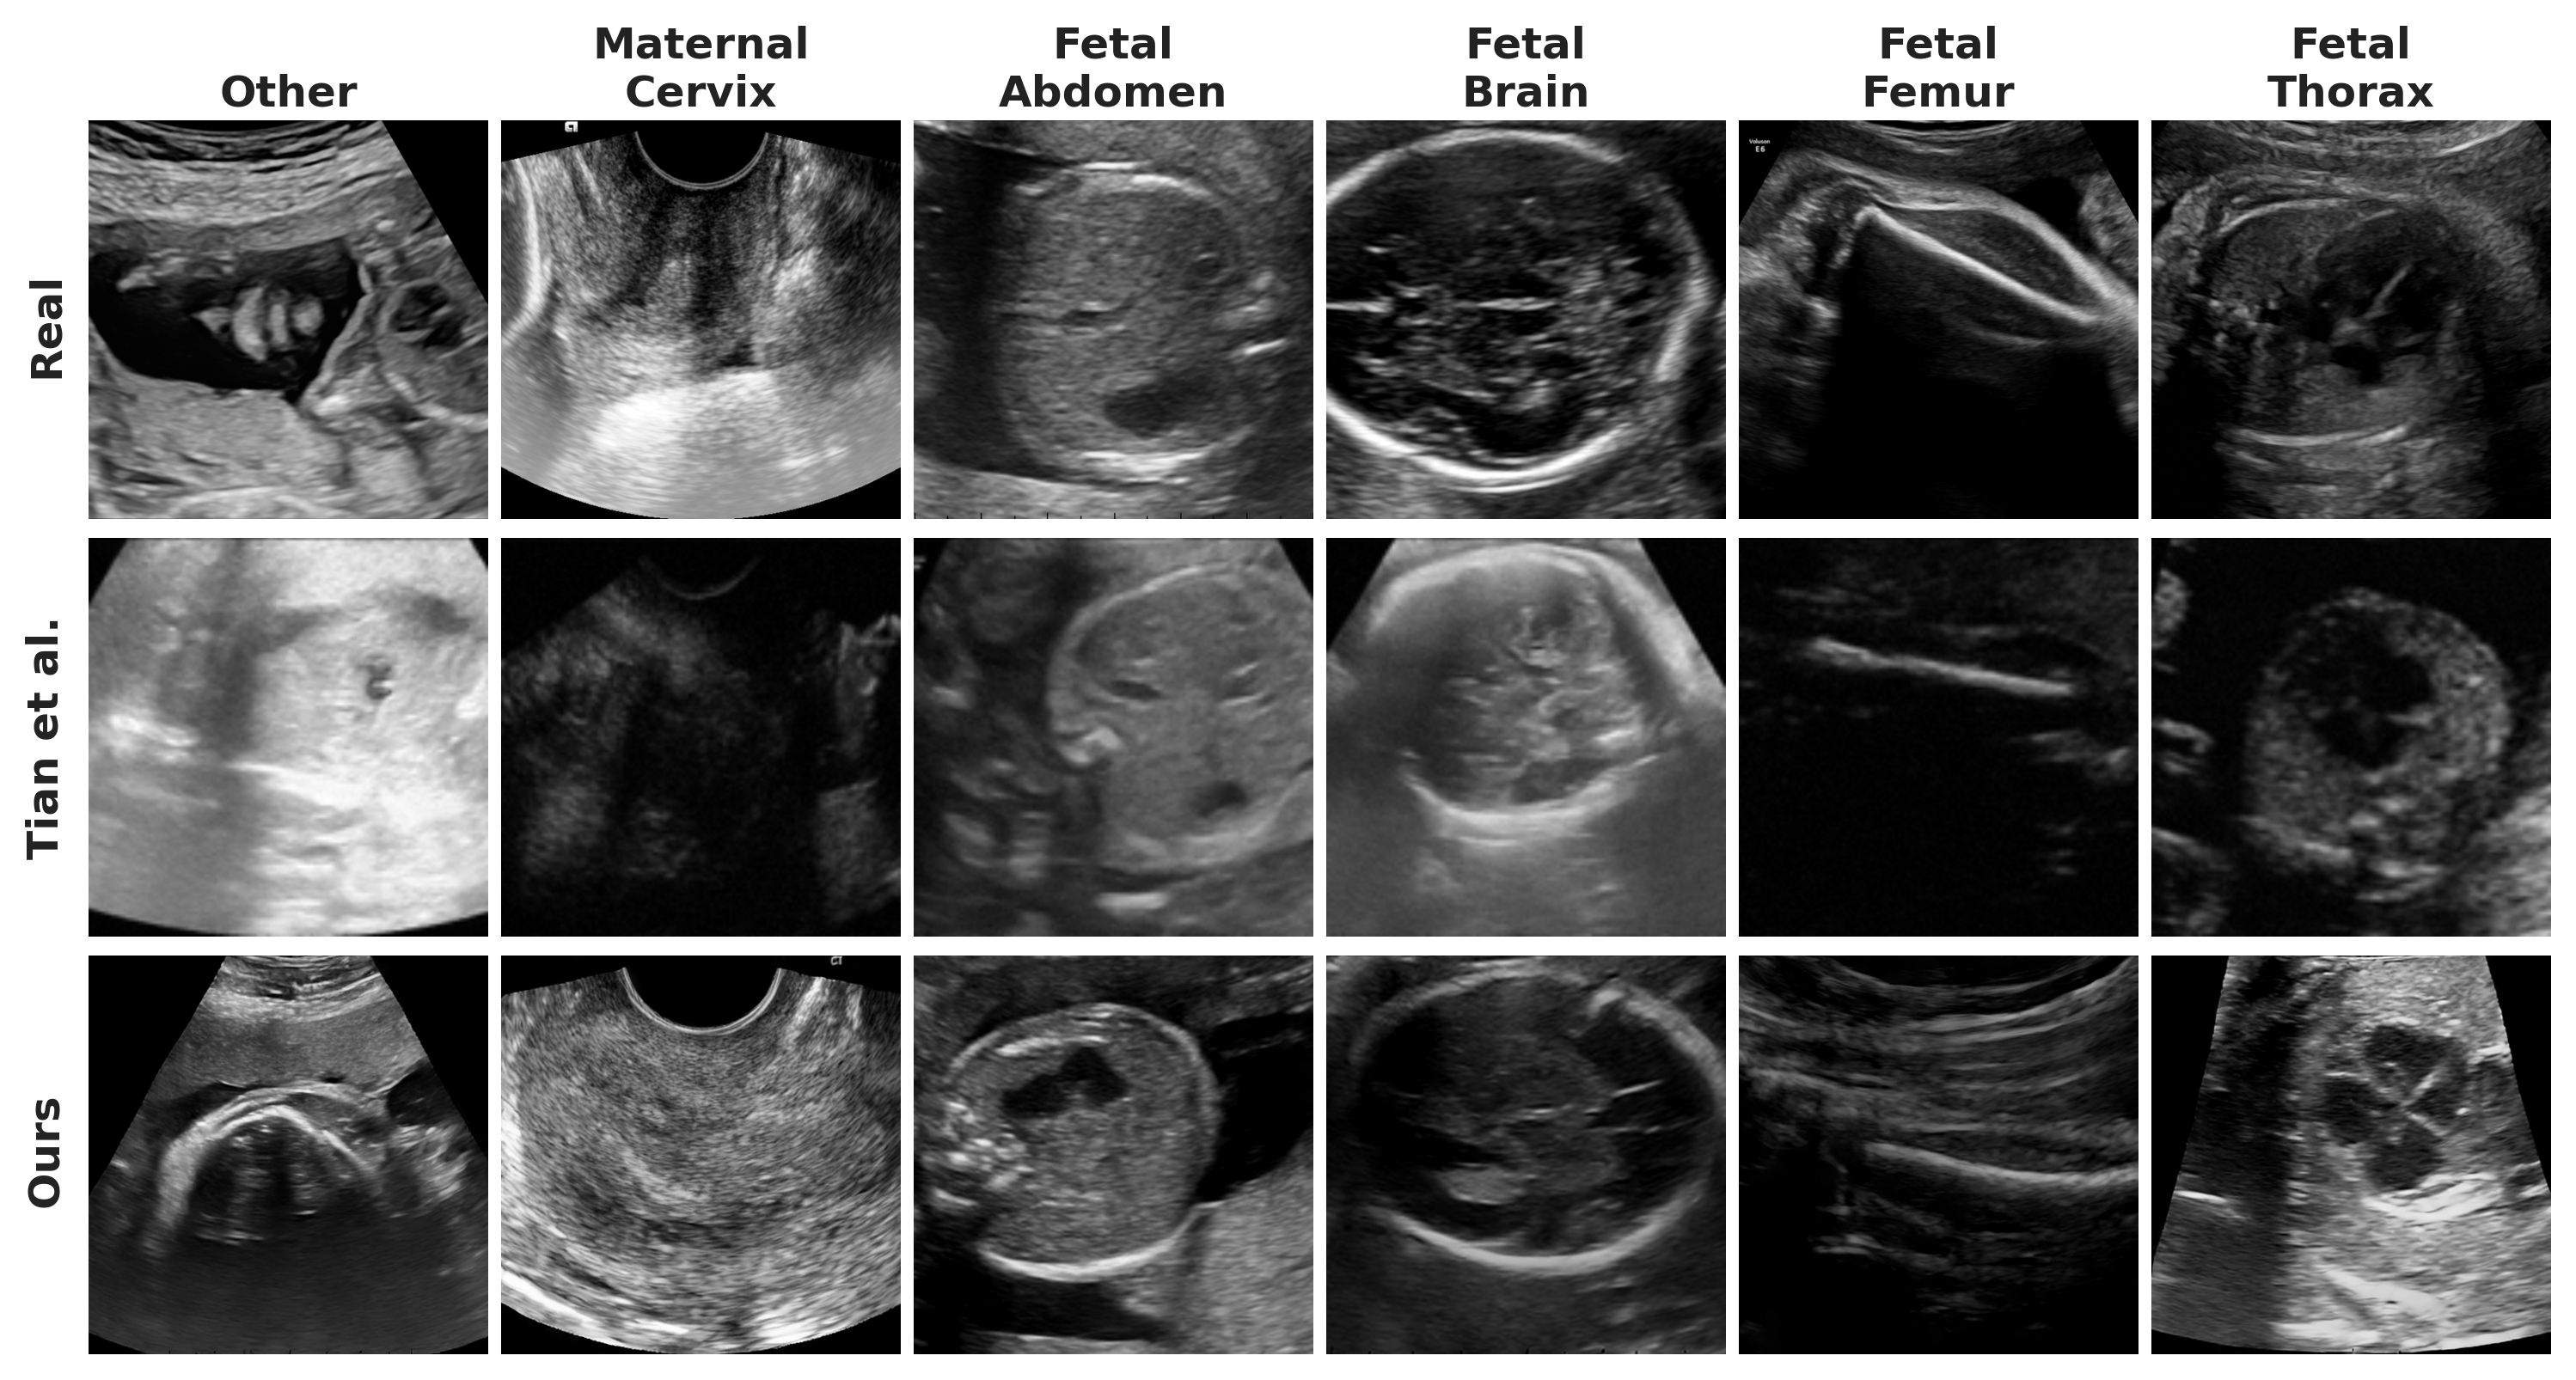
\includegraphics[width=0.4\linewidth]{image_grid.png}\label
  {fig:gen_images}

\vspace{-4mm}

\end{figure}

We evaluated the image quality of our image and compare them to \cite{tian2025enhancing} using Fréchet Inception Distance (FID) scores \cite{heusel2017gans}. We generate 5000 images for each of the six classes with a guidance scale of 2.25. For fair comparison, our images are downsized to 128 by 128. The results in Table \ref{tab:fid} show that our approach achieves higher quality in both individual classes and overall. Figure \ref{fig:gen_images} shows examples of generated images for each class.
Following Tian et al. \cite{tian2025enhancing}, who demonstrated that synthetic data improves fetal plane classification, we evaluated our high-resolution images using their top-performing architectures: ResNet50 \cite{he2016deep}, DenseNet169 \cite{huang2017densely}, and MedMamba \cite{yue2024medmamba}, plus a soft-voting ensemble. Using these specific models ensures a direct comparison with prior work.
%Tian et al. \cite{tian2025enhancing} showed that synthetic images could improve fetal plane classification performance. Building on this idea, we further evaluated the practical utility of our higher-resolution generated images through downstream fetal plane classification experiments using ResNet50, DenseNet169, and MedMamba, together with a soft-voting ensemble. These models were selected because they achieved the strongest classification performance in the evaluation reported by Tian et al., allowing a more direct comparison with prior work. 
We compared synthetic images generated by Tian et al. with our generated images under two settings: training from scratch on synthetic data only, and pretraining on synthetic data followed by real-world image fine-tuning. As shown in Table~\ref{tab:accuracy_comparison}, our images yielded stronger results when training from scratch, achieving 89.51\% ensemble accuracy. Under fine-tuning, our results also improved upon theirs, reaching a 93.36\% ensemble accuracy, surpassing the 92.32\% achieved on real-world data alone. These results suggest that our higher-resolution images are not only visually more realistic but also effective in supporting downstream classification performance.
%We compared synthetic images generated by Tian et al. with our generated images under two settings: training from scratch on synthetic data only, and pretraining on synthetic data followed by fine-tuning on real-world images. As shown in Table~\ref{tab:accuracy_comparison}, our generated images consistently yielded substantially stronger performance when training from scratch, achieving accuracies of 85.94\%, 87.67\%, and 86.34\% for ResNet50, DenseNet169, and MedMamba, respectively, with 89.51\% for the soft-voting ensemble, whereas classifiers trained on Tian et al.'s synthetic images performed poorly in this setting. Under fine-tuning, our results remained competitive and slightly improved over Tian et al. for most models, reaching 92.45\%, 92.15\%, and 91.77\%, with a soft-voting accuracy of 93.36\%. For reference, evaluation on the real-world FETAL\_PLANES\_DB dataset showed that the three individual models achieved accuracies above 90\%, while the ensemble reached 92.32\%. These results suggest that our higher-resolution synthetic images are not only visually more realistic, but also effective for supporting downstream classification with performance close to that obtained on real-world data.
%SURVEY
An experienced fetal ultrasound clinician (10 years’ expertise) evaluated 100 generated images, distinguishing real from synthetic and rating quality on a 5-point Likert scale. The mean score was 2.67, with real images scoring higher (3.12) than synthetic ones (2.07). Judgement relied on subtle artefacts including smoothing, speckle patterns, and anatomical inconsistencies.

\vspace{-5mm}
\begin{table}[htbp]
  \centering
  
  % --- First Table (Left) ---
  \begin{minipage}{0.4\textwidth}
    \centering
    \caption{FID comparison between Tian et al. \cite{tian2025enhancing} and our generated images.
    Lower FID indicates better image quality.}
    \label{tab:fid}
    \scriptsize
    \begin{tabular}{lcc}
      \toprule
      \bfseries Class & \bfseries Tian et al.  \cite{tian2025enhancing} & \bfseries Ours \\
      \midrule
      Other & 189.14 & \bf 143.30 \\
      Maternal cervix & 269.08 & \bf 155.30 \\
      Fetal abdomen & 241.14 & \bf 150.12 \\
      Fetal brain & 184.06 & \bf 117.71 \\
      Fetal femur & 203.10 & \bf 141.57 \\
      Fetal thorax & 233.37 & \bf 135.99 \\
      Overall & 176.85 & \bf 104.25 \\
      \bottomrule
    \end{tabular}
  \end{minipage}
  \hfill % Adds spacing between the two minipages
  % --- Second Table (Right) ---
  \begin{minipage}{0.56\textwidth}
    \centering
    \caption{Classifier accuracy comparison between Tian et al. \cite{tian2025enhancing} and our generated images.}
    \label{tab:accuracy_comparison}
    \scriptsize
    \begin{tabular}{llcc}
      \toprule
      \bfseries Method & \bfseries Model & \bfseries Tian et al. \cite{tian2025enhancing} & \bfseries Ours \\
      \midrule
      \multirow{4}{*}{\shortstack[l]{Training\\from\\Scratch}}
      & ResNet50     & 84.97\%  & \bf 85.94\% \\
      & DenseNet169  & 84.20\%  & \bf 87.67\% \\
      & MedMamba     & 82.53\%  & \bf 86.34\% \\
      & Soft Voting  & 87.35\%  & \bf 89.51\% \\
      \midrule
      \multirow{4}{*}{Fine-tuning}
      & ResNet50     & 91.29\% & \bf 92.45\% \\
      & DenseNet169  &  91.84\% & \bf 92.15\% \\
      & MedMamba     & 90.52\% & \bf 91.77\% \\
      & Soft Voting  & 92.84\% & \bf 93.36\% \\
      \bottomrule
    \end{tabular}
  \end{minipage}
\end{table}



\vspace{-12mm}
\section{Conclusions and future work}
We present an EDM2-based foundational model for high-resolution fetal ultrasound synthesis using open datasets, improving image quality and downstream classification performance. The model generates 512×512 images, surpassing prior 256×256 approaches. Clinical evaluation of 100 images yielded a mean score of 2.67/5, with real images rated higher than synthetic outputs. All code and models are released, with future work targeting scalable foundation models for low-resource healthcare and further comparison of diffusion architectures.

% \begin{credits}
% \subsubsection{\ackname} 
% This research was mainly supported by Studentship from the Faculty of Engineering and Physical Sciences - Electronic and Computer Science at the University of Southampton. The authors acknowledge the use of the IRIDIS X High Per- formance Computing Facility and the Southampton-Wolfson AI Research Machine (SWARM) GPU cluster, funded by the Wolfson Foundation, together with the associated support services at the University of Southampton in the completion of this work. The authors acknowledge the use of the UCL Unified AI Services Computing Facility (UAIServices@UCL), and associated support services, in the completion of this work.
% %%%%%%%%%%%%%%%%%%%%%%
% %UCL Unified AI
% % The authors acknowledge the use of the UCL Unified AI Services Computing Facility (UAIServices@UCL), and associated support services, in the completion of this work.


% \subsubsection{\discintname}
% The authors have no competing interests to declare that are relevant to the content of this article.
% % It is now necessary to declare any competing interests or to specifically
% % state that the authors have no competing interests. Please place the
% % statement with a bold run-in heading in small font size beneath the
% % (optional) acknowledgments\footnote{If EquinOCS, our proceedings submission
% % system, is used, then the disclaimer can be provided directly in the system.},
% % for example: The authors have no competing interests to declare that are
% % relevant to the content of this article. Or: Author A has received research
% % grants from Company W. Author B has received a speaker honorarium from
% % Company X and owns stock in Company Y. Author C is a member of committee Z.
% \end{credits}


%
% ---- Bibliography ----
%
% BibTeX users should specify bibliography style 'splncs04'.
% References will then be sorted and formatted in the correct style.
%
\bibliographystyle{splncs04}
%\bibliography{mybibliography}%%%OVERLEAF
\bibliography{../../latex/mybibliography}%%%GITHUB/ARXIV
% % This is samplepaper.tex, a sample chapter demonstrating the
% LLNCS macro package for Springer Computer Science proceedings;
% Version 2.21 of 2022/01/12
%


% Camera-ready submissions: All accepted papers must follow the below guidelines to submit your camera-ready papers –

% Your paper should contain your full authors names, full affiliation and ORCID ID (if available). Your submission should contain source files (e.g., latex files or word document). Please read the "Instructions for proceedings authors.pdf" carefully and make sure that you follow these instructions. The link is provided here: (opens in a new window)Instructions for proceedings authors.
% You should print, sign, and scan the "Licence to Publish Proceedings Papers". The license will be provided upon notification of acceptance. 
% Short papers: Authors are invited to submit short papers of length up to 3 pages excluding references (1 column – the LNCS template) showing proof-of-concept research contributions under the topics of the conference. All submissions will be peer-reviewed and the accepted abstracts will be published in Frontiers in Medical Technology as an ebook. Please use the template provided below.

% The word and character limits per short paper are as follows:
% -Title: 500 characters
% -Text: 1,000 words
% -Figures: 2
% -No Supplementary Material

% MIUA continues to foster fairness, diversity, and inclusion within its community. Submissions from typically underrepresented groups are particularly encouraged.

% https://www.ucd.ie/medicine/miua2026/calls/callforpapers/

% Reviewer #1
% Questions
% 1. Please provide major strengths of the paper.
% The paper presents a fetal ultrasound synthesis framework and shows that models trained on the proposed dataset achieve better performance than those trained on datasets used in previous work.

% 2. Please provide any major weaknesses of the paper.
% Although this is a short paper, the technical contribution appears weak. The proposed method is based on the existing EDM2 latent diffusion model, and the paper provides very limited implementation details, with no description of the training configuration beyond the loss function.


% 3. Overall evaluation of the paper.
% Accept


% 6. Constructive feedback to authors for improving the paper. (optional)
% It would be useful to include results from different network architectures trained on the same dataset with identical training configurations. The current version does not clearly demonstrate whether the observed performance is attributable to the EDM2 architecture or to the dataset used for training.

% KEY DATES
% Full Paper Submission: Thursday 2nd April 2026 (01:00 Pacific Time (PT))
% Notification of Acceptance: Friday 5th June 2026 
% Camera Ready Deadline: Friday 12th June 2026
% Early Registration: Friday 12th June 2026





\documentclass[runningheads]{llncs}
%
\usepackage[T1]{fontenc}
% T1 fonts will be used to generate the final print and online PDFs,
% so please use T1 fonts in your manuscript whenever possible.
% Other font encondings may result in incorrect characters.
%
\usepackage{booktabs} 
\usepackage{graphicx}
\usepackage{multirow}
\usepackage{orcidlink}
% Used for displaying a sample figure. If possible, figure files should
% be included in EPS format.
%
% If you use the hyperref package, please uncomment the following two lines
% to display URLs in blue roman font according to Springer's eBook style:
%\usepackage{color}
%\renewcommand\UrlFont{\color{blue}\rmfamily}
%\urlstyle{rm}

\vspace{-10mm}

\begin{document}
\title{
A Foundational EDM2-Based Generative Model for High-Resolution Synthetic Fetal Ultrasound Imaging from Open Datasets
}
%
%\titlerunning{Abbreviated paper title}
% If the paper title is too long for the running head, you can set
% an abbreviated paper title here
%

%\author{Anonymous Author(s)}

%\authorrunning{Anonymous Author(s)}
% First names are abbreviated in the running head.
% If there are more than two authors, 'et al.' is used.
%
%\institute{Affiliation(s)}

\author{Harvey Mannering\inst{1}\orcidlink{0000-0003-3094-7417} \and
Yilin Zhang\inst{1}\orcidlink{0009-0008-3660-5737}  \and
Ziao Liu\inst{2}\orcidlink{0009-0006-1905-1061} \and
Zhiwu Huang \inst{1}\orcidlink{0000-0002-7385-079X} \and
Jacqueline Matthew\inst{3}\orcidlink{0000-0003-4754-0322} \and
Miguel Xochicale\inst{4}\orcidlink{0000-0002-8225-7517}}


\authorrunning{H. Mannering et al.}
\titlerunning{EDM2-Based Fetal Ultrasound Generation}
% % First names are abbreviated in the running head.
% % If there are more than two authors, 'et al.' is used.
% %
\institute{
$^1$ University of Southampton,
$^2$ Tsinghua University,
$^3$ King's College London, \\
$^4$ University College London
\thanks{
Work on diffusion models with the U. of Southampton supported by PhD studentship, Tsinghua University (classification), KCL (clinical evaluation) and reproducible workflows and robust software engineering on UCL-ARC’s Unified-AI cloud platform.
}
}


\maketitle              % typeset the header of the contribution

\vspace{-5mm}
% The abstract should briefly summarize the contents of the paper in 150--250 words.
\begin{abstract}
Prenatal ultrasound imaging is key for assessing fetal health, but AI progress is limited by scarce, privacy-restricted, and hard-to-annotate datasets. 
We propose a high-resolution fetal ultrasound synthesis framework based on the EDM2 diffusion architecture, trained on multiple public datasets to generate 512×512 images across six anatomical classes. Our method achieved improved image quality with lower FID scores and enhanced downstream fetal plane classification, reaching 93.36\% ensemble accuracy after fine-tuning, surpassing real-data-only training. 
Clinical evaluation by an experienced fetal ultrasound specialist (10+ years) on 100 images yielded a mean realism score of 2.67/5, with real images rated higher than synthetic. Artefacts included smoothing, speckle irregularities, and anatomical inconsistencies. 
Code, data, models and other resources to reproduce this work are available at \url{https://github.com/xfetus/fetal-ultrasound-edm2}.
\keywords{
Fetal Ultrasound \and 
% Diffusion Models \and 
Synthetic Medical Imaging
}
\end{abstract}


\vspace{-9mm}
\section{Introduction}
Prenatal ultrasound (US) imaging is the primary modality for assessing fetal health and development. Recent advances in AI have accelerated the development of classifiers, automated detection systems, and synthetic image generation methods for prenatal imaging. However, clinically reliable AI models require diverse datasets that capture real-world complexity, including varied fetal conditions, US scanners, patient demographics, and imaging modalities from 2D to emerging 3D-4D US \cite{kurjak2007useful}. Additional challenges include inconsistent volumetric assessment protocols, operator-dependent variability between sonographers, and natural anatomical variation between patients and fetuses \cite{jcm13185626}. 
Open datasets and evaluation frameworks are therefore essential for assessing AI model fidelity, robustness, and diversity \cite{IBRAHIM2025}.
Recently, \cite{Alsharid2025} published a comprehensive overview of publicly available US resources, including datasets and deep learning models, which is highly relevant to open-source strategies in US imaging. 
However, fetal US datasets remain largely centred on the FETAL PLANES DB, which contains 12,400 images \cite{burgos2020evaluation}. \cite{Alsharid2025} also reports additional emerging datasets, including the US Fetus Phantom dataset (15,728 images), the Fetal Head dataset (1,334 images), the Fetal Abdomen dataset (4,668 images), and the Fetal Cardiac dataset (300 images).
Parallel to this work, generative models such as GANs \cite{Goodfellow2014}, VAE \cite{kingma2013auto}, diffusion models \cite{ho2020_neurips}, and flow-based models \cite{lipman2022flow} are now a promising avenue to address data scarcity in medical images \cite{yan2018generation,tian2025enhancing}.
Diffusion-Based Fetal US Synthesis with Active Learning presented promising results on image quality comparison with baseline models but no clinical evaluation is included \cite{Arjemandi2026}. In US images, Stable Diffusion 1.5 \cite{rombach2022high} with ControlNet \cite{zhang2023adding} has enabled localized tumor synthesis \cite{freiche2025ultrasound}, while Tian et al. \cite{tian2025enhancing} utilized diffusion-generated images to improve plane classification, although only at $128 \times 128$ resolution. While hybrid Diffusion-GAN approaches \cite{iskandar2023towards} reached $256 \times 256$, these resolutions remain clinically restrictive and rely on older architectures. By contrast, we apply EDM2 \cite{karras2024analyzing}, the current state of the art for ImageNet generation \cite{deng2009imagenet}, to synthesize high-fidelity fetal US images at a more realistic $512 \times 512$ resolution.

%%%%%%%%%%%%%%%%%%%%%%%%%%%%%%%%%%%%%%%%%%%%%%%%%%%%%%%%%%%%%%%%%%%%%%%%%%%%%
%%%%%%%%%%%%%%%%%%%%%%%%%%%%%%%%%%%%%%%%%%%%%%%%%%%%%%%%%%%%%%%%%%%%%%%%%%%%%
%%%%%%%%%%%%%%%%%%%%%%%%%%%%%%%%%%%%%%%%%%%%%%%%%%%%%%%%%%%%%%%%%%%%%%%%%%%%%
\section{Methods and datasets}

We trained the EDM2 diffusion model to generate 6 US images classes with center cropping, random horizontal flipping, and resizing to $512 \times 512$, following the training setup from \cite{tian2025enhancing}, except with a higher resolution. We train two different sized networks, EDM2-S and EDM2-XL, which allows us to apply autoguidance \cite{karras2024guiding} to improve image quality.
We focus on the FETAL PLANES DB dataset (12,400 images) \cite{burgos2020evaluation}, which includes six classes: maternal cervix, fetal abdomen, fetal brain, fetal femur, fetal thorax, and other.
However, this dataset is relatively small, there is a risk of the diffusion model memorizing training data.
To mitigate this, we incorporate additional datasets: the FPU23 dataset (15,728 images) \cite{prabakaran2023fpus23}, a fetal abdominal structures segmentation dataset (1,588 images) \cite{da2023fetal}, and an African low-resource dataset (451 images) \cite{sendra2023generalisability}.
Each additional dataset is given a single label during training. 
We use a weighted MSE loss, weighting FETAL PLANES DB at 2.0 and others at 1.0.
Including these datasets allows twice as many training steps and reduces validation loss from 0.1427 to 0.1371.

\section{Experiments and results}

\begin{figure}[htbp]
\centering
  \caption{
  Representative fetal ultrasound images from real data, Tian et al. \cite{tian2025enhancing}, and our proposed high-resolution ($512 \times 512$) diffusion-based synthesis approach.
  Higher resolution image at our repository  \url{https://github.com/xfetus/fetal-ultrasound-edm2}.
  }
  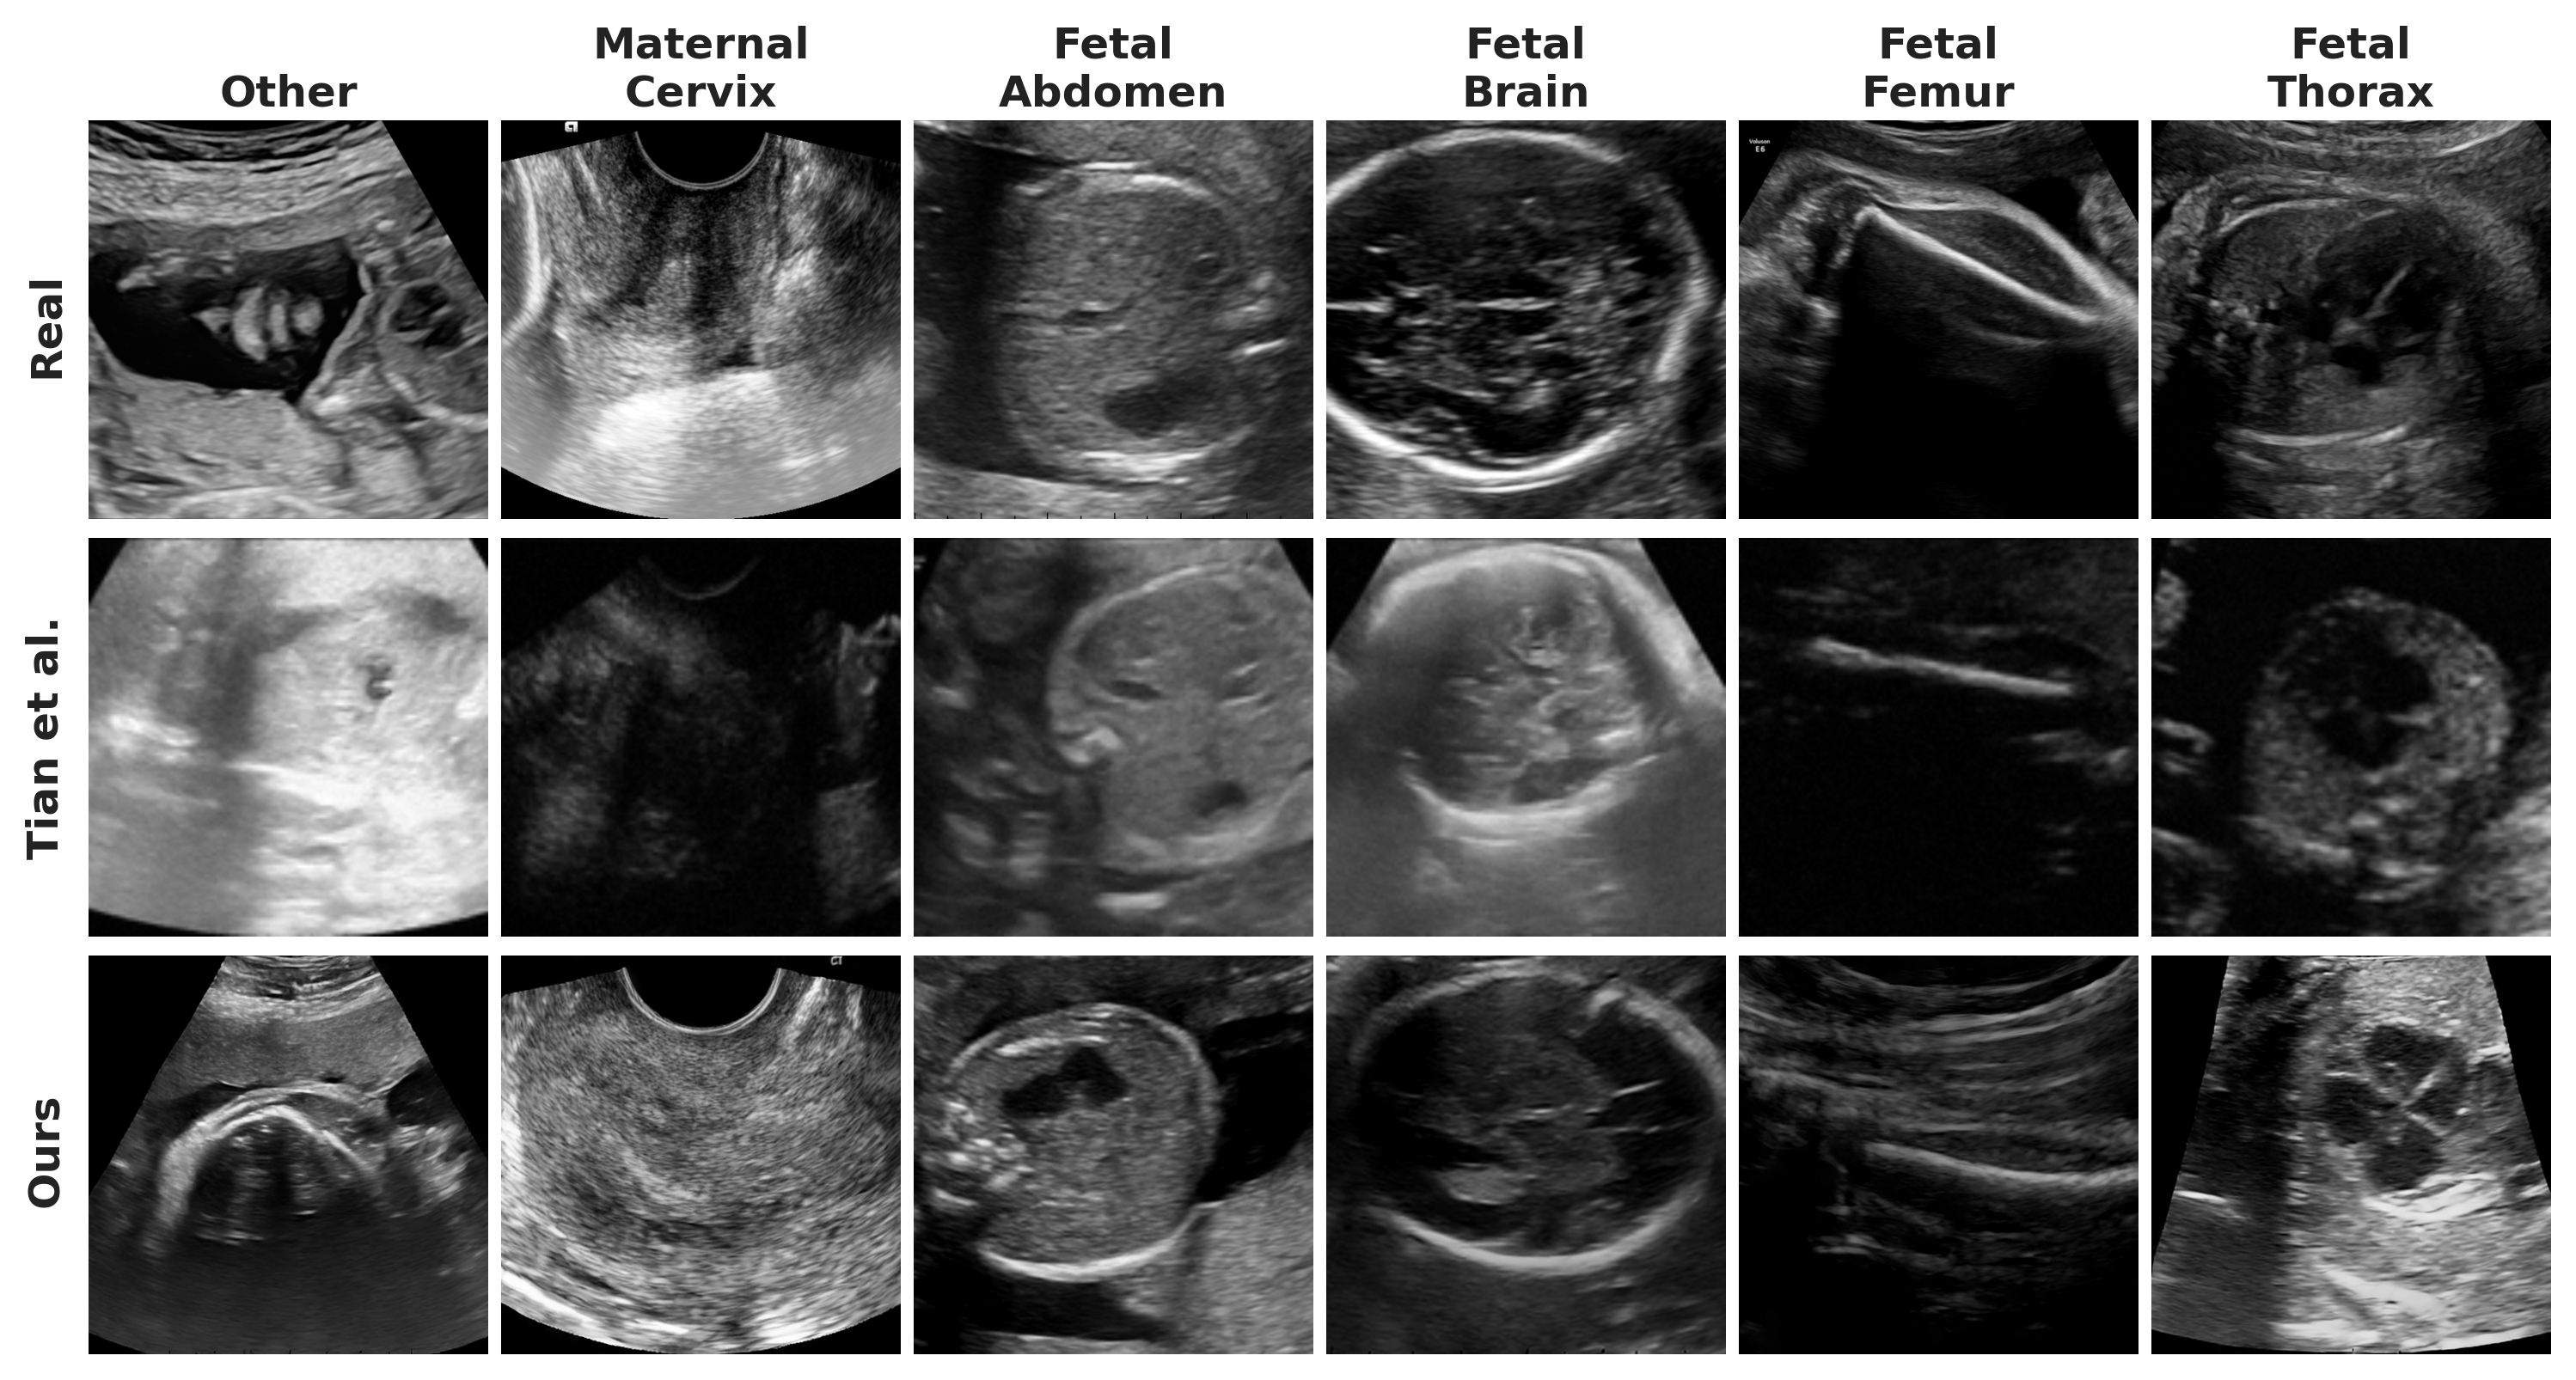
\includegraphics[width=0.4\linewidth]{image_grid.png}\label
  {fig:gen_images}

\vspace{-4mm}

\end{figure}

We evaluated the image quality of our image and compare them to \cite{tian2025enhancing} using Fréchet Inception Distance (FID) scores \cite{heusel2017gans}. We generate 5000 images for each of the six classes with a guidance scale of 2.25. For fair comparison, our images are downsized to 128 by 128. The results in Table \ref{tab:fid} show that our approach achieves higher quality in both individual classes and overall. Figure \ref{fig:gen_images} shows examples of generated images for each class.
Following Tian et al. \cite{tian2025enhancing}, who demonstrated that synthetic data improves fetal plane classification, we evaluated our high-resolution images using their top-performing architectures: ResNet50 \cite{he2016deep}, DenseNet169 \cite{huang2017densely}, and MedMamba \cite{yue2024medmamba}, plus a soft-voting ensemble. Using these specific models ensures a direct comparison with prior work.
%Tian et al. \cite{tian2025enhancing} showed that synthetic images could improve fetal plane classification performance. Building on this idea, we further evaluated the practical utility of our higher-resolution generated images through downstream fetal plane classification experiments using ResNet50, DenseNet169, and MedMamba, together with a soft-voting ensemble. These models were selected because they achieved the strongest classification performance in the evaluation reported by Tian et al., allowing a more direct comparison with prior work. 
We compared synthetic images generated by Tian et al. with our generated images under two settings: training from scratch on synthetic data only, and pretraining on synthetic data followed by real-world image fine-tuning. As shown in Table~\ref{tab:accuracy_comparison}, our images yielded stronger results when training from scratch, achieving 89.51\% ensemble accuracy. Under fine-tuning, our results also improved upon theirs, reaching a 93.36\% ensemble accuracy, surpassing the 92.32\% achieved on real-world data alone. These results suggest that our higher-resolution images are not only visually more realistic but also effective in supporting downstream classification performance.
%We compared synthetic images generated by Tian et al. with our generated images under two settings: training from scratch on synthetic data only, and pretraining on synthetic data followed by fine-tuning on real-world images. As shown in Table~\ref{tab:accuracy_comparison}, our generated images consistently yielded substantially stronger performance when training from scratch, achieving accuracies of 85.94\%, 87.67\%, and 86.34\% for ResNet50, DenseNet169, and MedMamba, respectively, with 89.51\% for the soft-voting ensemble, whereas classifiers trained on Tian et al.'s synthetic images performed poorly in this setting. Under fine-tuning, our results remained competitive and slightly improved over Tian et al. for most models, reaching 92.45\%, 92.15\%, and 91.77\%, with a soft-voting accuracy of 93.36\%. For reference, evaluation on the real-world FETAL\_PLANES\_DB dataset showed that the three individual models achieved accuracies above 90\%, while the ensemble reached 92.32\%. These results suggest that our higher-resolution synthetic images are not only visually more realistic, but also effective for supporting downstream classification with performance close to that obtained on real-world data.
%SURVEY
An experienced fetal ultrasound clinician (10 years’ expertise) evaluated 100 generated images, distinguishing real from synthetic and rating quality on a 5-point Likert scale. The mean score was 2.67, with real images scoring higher (3.12) than synthetic ones (2.07). Judgement relied on subtle artefacts including smoothing, speckle patterns, and anatomical inconsistencies.

\vspace{-5mm}
\begin{table}[htbp]
  \centering
  
  % --- First Table (Left) ---
  \begin{minipage}{0.4\textwidth}
    \centering
    \caption{FID comparison between Tian et al. \cite{tian2025enhancing} and our generated images.
    Lower FID indicates better image quality.}
    \label{tab:fid}
    \scriptsize
    \begin{tabular}{lcc}
      \toprule
      \bfseries Class & \bfseries Tian et al.  \cite{tian2025enhancing} & \bfseries Ours \\
      \midrule
      Other & 189.14 & \bf 143.30 \\
      Maternal cervix & 269.08 & \bf 155.30 \\
      Fetal abdomen & 241.14 & \bf 150.12 \\
      Fetal brain & 184.06 & \bf 117.71 \\
      Fetal femur & 203.10 & \bf 141.57 \\
      Fetal thorax & 233.37 & \bf 135.99 \\
      Overall & 176.85 & \bf 104.25 \\
      \bottomrule
    \end{tabular}
  \end{minipage}
  \hfill % Adds spacing between the two minipages
  % --- Second Table (Right) ---
  \begin{minipage}{0.56\textwidth}
    \centering
    \caption{Classifier accuracy comparison between Tian et al. \cite{tian2025enhancing} and our generated images.}
    \label{tab:accuracy_comparison}
    \scriptsize
    \begin{tabular}{llcc}
      \toprule
      \bfseries Method & \bfseries Model & \bfseries Tian et al. \cite{tian2025enhancing} & \bfseries Ours \\
      \midrule
      \multirow{4}{*}{\shortstack[l]{Training\\from\\Scratch}}
      & ResNet50     & 84.97\%  & \bf 85.94\% \\
      & DenseNet169  & 84.20\%  & \bf 87.67\% \\
      & MedMamba     & 82.53\%  & \bf 86.34\% \\
      & Soft Voting  & 87.35\%  & \bf 89.51\% \\
      \midrule
      \multirow{4}{*}{Fine-tuning}
      & ResNet50     & 91.29\% & \bf 92.45\% \\
      & DenseNet169  &  91.84\% & \bf 92.15\% \\
      & MedMamba     & 90.52\% & \bf 91.77\% \\
      & Soft Voting  & 92.84\% & \bf 93.36\% \\
      \bottomrule
    \end{tabular}
  \end{minipage}
\end{table}



\vspace{-12mm}
\section{Conclusions and future work}
We present an EDM2-based foundational model for high-resolution fetal ultrasound synthesis using open datasets, improving image quality and downstream classification performance. The model generates 512×512 images, surpassing prior 256×256 approaches. Clinical evaluation of 100 images yielded a mean score of 2.67/5, with real images rated higher than synthetic outputs. All code and models are released, with future work targeting scalable foundation models for low-resource healthcare and further comparison of diffusion architectures.

% \begin{credits}
% \subsubsection{\ackname} 
% This research was mainly supported by Studentship from the Faculty of Engineering and Physical Sciences - Electronic and Computer Science at the University of Southampton. The authors acknowledge the use of the IRIDIS X High Per- formance Computing Facility and the Southampton-Wolfson AI Research Machine (SWARM) GPU cluster, funded by the Wolfson Foundation, together with the associated support services at the University of Southampton in the completion of this work. The authors acknowledge the use of the UCL Unified AI Services Computing Facility (UAIServices@UCL), and associated support services, in the completion of this work.
% %%%%%%%%%%%%%%%%%%%%%%
% %UCL Unified AI
% % The authors acknowledge the use of the UCL Unified AI Services Computing Facility (UAIServices@UCL), and associated support services, in the completion of this work.


% \subsubsection{\discintname}
% The authors have no competing interests to declare that are relevant to the content of this article.
% % It is now necessary to declare any competing interests or to specifically
% % state that the authors have no competing interests. Please place the
% % statement with a bold run-in heading in small font size beneath the
% % (optional) acknowledgments\footnote{If EquinOCS, our proceedings submission
% % system, is used, then the disclaimer can be provided directly in the system.},
% % for example: The authors have no competing interests to declare that are
% % relevant to the content of this article. Or: Author A has received research
% % grants from Company W. Author B has received a speaker honorarium from
% % Company X and owns stock in Company Y. Author C is a member of committee Z.
% \end{credits}


%
% ---- Bibliography ----
%
% BibTeX users should specify bibliography style 'splncs04'.
% References will then be sorted and formatted in the correct style.
%
\bibliographystyle{splncs04}
%\bibliography{mybibliography}%%%OVERLEAF
\bibliography{../../latex/mybibliography}%%%GITHUB/ARXIV
% % This is samplepaper.tex, a sample chapter demonstrating the
% LLNCS macro package for Springer Computer Science proceedings;
% Version 2.21 of 2022/01/12
%


% Camera-ready submissions: All accepted papers must follow the below guidelines to submit your camera-ready papers –

% Your paper should contain your full authors names, full affiliation and ORCID ID (if available). Your submission should contain source files (e.g., latex files or word document). Please read the "Instructions for proceedings authors.pdf" carefully and make sure that you follow these instructions. The link is provided here: (opens in a new window)Instructions for proceedings authors.
% You should print, sign, and scan the "Licence to Publish Proceedings Papers". The license will be provided upon notification of acceptance. 
% Short papers: Authors are invited to submit short papers of length up to 3 pages excluding references (1 column – the LNCS template) showing proof-of-concept research contributions under the topics of the conference. All submissions will be peer-reviewed and the accepted abstracts will be published in Frontiers in Medical Technology as an ebook. Please use the template provided below.

% The word and character limits per short paper are as follows:
% -Title: 500 characters
% -Text: 1,000 words
% -Figures: 2
% -No Supplementary Material

% MIUA continues to foster fairness, diversity, and inclusion within its community. Submissions from typically underrepresented groups are particularly encouraged.

% https://www.ucd.ie/medicine/miua2026/calls/callforpapers/

% Reviewer #1
% Questions
% 1. Please provide major strengths of the paper.
% The paper presents a fetal ultrasound synthesis framework and shows that models trained on the proposed dataset achieve better performance than those trained on datasets used in previous work.

% 2. Please provide any major weaknesses of the paper.
% Although this is a short paper, the technical contribution appears weak. The proposed method is based on the existing EDM2 latent diffusion model, and the paper provides very limited implementation details, with no description of the training configuration beyond the loss function.


% 3. Overall evaluation of the paper.
% Accept


% 6. Constructive feedback to authors for improving the paper. (optional)
% It would be useful to include results from different network architectures trained on the same dataset with identical training configurations. The current version does not clearly demonstrate whether the observed performance is attributable to the EDM2 architecture or to the dataset used for training.

% KEY DATES
% Full Paper Submission: Thursday 2nd April 2026 (01:00 Pacific Time (PT))
% Notification of Acceptance: Friday 5th June 2026 
% Camera Ready Deadline: Friday 12th June 2026
% Early Registration: Friday 12th June 2026





\documentclass[runningheads]{llncs}
%
\usepackage[T1]{fontenc}
% T1 fonts will be used to generate the final print and online PDFs,
% so please use T1 fonts in your manuscript whenever possible.
% Other font encondings may result in incorrect characters.
%
\usepackage{booktabs} 
\usepackage{graphicx}
\usepackage{multirow}
\usepackage{orcidlink}
% Used for displaying a sample figure. If possible, figure files should
% be included in EPS format.
%
% If you use the hyperref package, please uncomment the following two lines
% to display URLs in blue roman font according to Springer's eBook style:
%\usepackage{color}
%\renewcommand\UrlFont{\color{blue}\rmfamily}
%\urlstyle{rm}

\vspace{-10mm}

\begin{document}
\title{
A Foundational EDM2-Based Generative Model for High-Resolution Synthetic Fetal Ultrasound Imaging from Open Datasets
}
%
%\titlerunning{Abbreviated paper title}
% If the paper title is too long for the running head, you can set
% an abbreviated paper title here
%

%\author{Anonymous Author(s)}

%\authorrunning{Anonymous Author(s)}
% First names are abbreviated in the running head.
% If there are more than two authors, 'et al.' is used.
%
%\institute{Affiliation(s)}

\author{Harvey Mannering\inst{1}\orcidlink{0000-0003-3094-7417} \and
Yilin Zhang\inst{1}\orcidlink{0009-0008-3660-5737}  \and
Ziao Liu\inst{2}\orcidlink{0009-0006-1905-1061} \and
Zhiwu Huang \inst{1}\orcidlink{0000-0002-7385-079X} \and
Jacqueline Matthew\inst{3}\orcidlink{0000-0003-4754-0322} \and
Miguel Xochicale\inst{4}\orcidlink{0000-0002-8225-7517}}


\authorrunning{H. Mannering et al.}
\titlerunning{EDM2-Based Fetal Ultrasound Generation}
% % First names are abbreviated in the running head.
% % If there are more than two authors, 'et al.' is used.
% %
\institute{
$^1$ University of Southampton,
$^2$ Tsinghua University,
$^3$ King's College London, \\
$^4$ University College London
\thanks{
Work on diffusion models with the U. of Southampton supported by PhD studentship, Tsinghua University (classification), KCL (clinical evaluation) and reproducible workflows and robust software engineering on UCL-ARC’s Unified-AI cloud platform.
}
}


\maketitle              % typeset the header of the contribution

\vspace{-5mm}
% The abstract should briefly summarize the contents of the paper in 150--250 words.
\begin{abstract}
Prenatal ultrasound imaging is key for assessing fetal health, but AI progress is limited by scarce, privacy-restricted, and hard-to-annotate datasets. 
We propose a high-resolution fetal ultrasound synthesis framework based on the EDM2 diffusion architecture, trained on multiple public datasets to generate 512×512 images across six anatomical classes. Our method achieved improved image quality with lower FID scores and enhanced downstream fetal plane classification, reaching 93.36\% ensemble accuracy after fine-tuning, surpassing real-data-only training. 
Clinical evaluation by an experienced fetal ultrasound specialist (10+ years) on 100 images yielded a mean realism score of 2.67/5, with real images rated higher than synthetic. Artefacts included smoothing, speckle irregularities, and anatomical inconsistencies. 
Code, data, models and other resources to reproduce this work are available at \url{https://github.com/xfetus/fetal-ultrasound-edm2}.
\keywords{
Fetal Ultrasound \and 
% Diffusion Models \and 
Synthetic Medical Imaging
}
\end{abstract}


\vspace{-9mm}
\section{Introduction}
Prenatal ultrasound (US) imaging is the primary modality for assessing fetal health and development. Recent advances in AI have accelerated the development of classifiers, automated detection systems, and synthetic image generation methods for prenatal imaging. However, clinically reliable AI models require diverse datasets that capture real-world complexity, including varied fetal conditions, US scanners, patient demographics, and imaging modalities from 2D to emerging 3D-4D US \cite{kurjak2007useful}. Additional challenges include inconsistent volumetric assessment protocols, operator-dependent variability between sonographers, and natural anatomical variation between patients and fetuses \cite{jcm13185626}. 
Open datasets and evaluation frameworks are therefore essential for assessing AI model fidelity, robustness, and diversity \cite{IBRAHIM2025}.
Recently, \cite{Alsharid2025} published a comprehensive overview of publicly available US resources, including datasets and deep learning models, which is highly relevant to open-source strategies in US imaging. 
However, fetal US datasets remain largely centred on the FETAL PLANES DB, which contains 12,400 images \cite{burgos2020evaluation}. \cite{Alsharid2025} also reports additional emerging datasets, including the US Fetus Phantom dataset (15,728 images), the Fetal Head dataset (1,334 images), the Fetal Abdomen dataset (4,668 images), and the Fetal Cardiac dataset (300 images).
Parallel to this work, generative models such as GANs \cite{Goodfellow2014}, VAE \cite{kingma2013auto}, diffusion models \cite{ho2020_neurips}, and flow-based models \cite{lipman2022flow} are now a promising avenue to address data scarcity in medical images \cite{yan2018generation,tian2025enhancing}.
Diffusion-Based Fetal US Synthesis with Active Learning presented promising results on image quality comparison with baseline models but no clinical evaluation is included \cite{Arjemandi2026}. In US images, Stable Diffusion 1.5 \cite{rombach2022high} with ControlNet \cite{zhang2023adding} has enabled localized tumor synthesis \cite{freiche2025ultrasound}, while Tian et al. \cite{tian2025enhancing} utilized diffusion-generated images to improve plane classification, although only at $128 \times 128$ resolution. While hybrid Diffusion-GAN approaches \cite{iskandar2023towards} reached $256 \times 256$, these resolutions remain clinically restrictive and rely on older architectures. By contrast, we apply EDM2 \cite{karras2024analyzing}, the current state of the art for ImageNet generation \cite{deng2009imagenet}, to synthesize high-fidelity fetal US images at a more realistic $512 \times 512$ resolution.

%%%%%%%%%%%%%%%%%%%%%%%%%%%%%%%%%%%%%%%%%%%%%%%%%%%%%%%%%%%%%%%%%%%%%%%%%%%%%
%%%%%%%%%%%%%%%%%%%%%%%%%%%%%%%%%%%%%%%%%%%%%%%%%%%%%%%%%%%%%%%%%%%%%%%%%%%%%
%%%%%%%%%%%%%%%%%%%%%%%%%%%%%%%%%%%%%%%%%%%%%%%%%%%%%%%%%%%%%%%%%%%%%%%%%%%%%
\section{Methods and datasets}

We trained the EDM2 diffusion model to generate 6 US images classes with center cropping, random horizontal flipping, and resizing to $512 \times 512$, following the training setup from \cite{tian2025enhancing}, except with a higher resolution. We train two different sized networks, EDM2-S and EDM2-XL, which allows us to apply autoguidance \cite{karras2024guiding} to improve image quality.
We focus on the FETAL PLANES DB dataset (12,400 images) \cite{burgos2020evaluation}, which includes six classes: maternal cervix, fetal abdomen, fetal brain, fetal femur, fetal thorax, and other.
However, this dataset is relatively small, there is a risk of the diffusion model memorizing training data.
To mitigate this, we incorporate additional datasets: the FPU23 dataset (15,728 images) \cite{prabakaran2023fpus23}, a fetal abdominal structures segmentation dataset (1,588 images) \cite{da2023fetal}, and an African low-resource dataset (451 images) \cite{sendra2023generalisability}.
Each additional dataset is given a single label during training. 
We use a weighted MSE loss, weighting FETAL PLANES DB at 2.0 and others at 1.0.
Including these datasets allows twice as many training steps and reduces validation loss from 0.1427 to 0.1371.

\section{Experiments and results}

\begin{figure}[htbp]
\centering
  \caption{
  Representative fetal ultrasound images from real data, Tian et al. \cite{tian2025enhancing}, and our proposed high-resolution ($512 \times 512$) diffusion-based synthesis approach.
  Higher resolution image at our repository  \url{https://github.com/xfetus/fetal-ultrasound-edm2}.
  }
  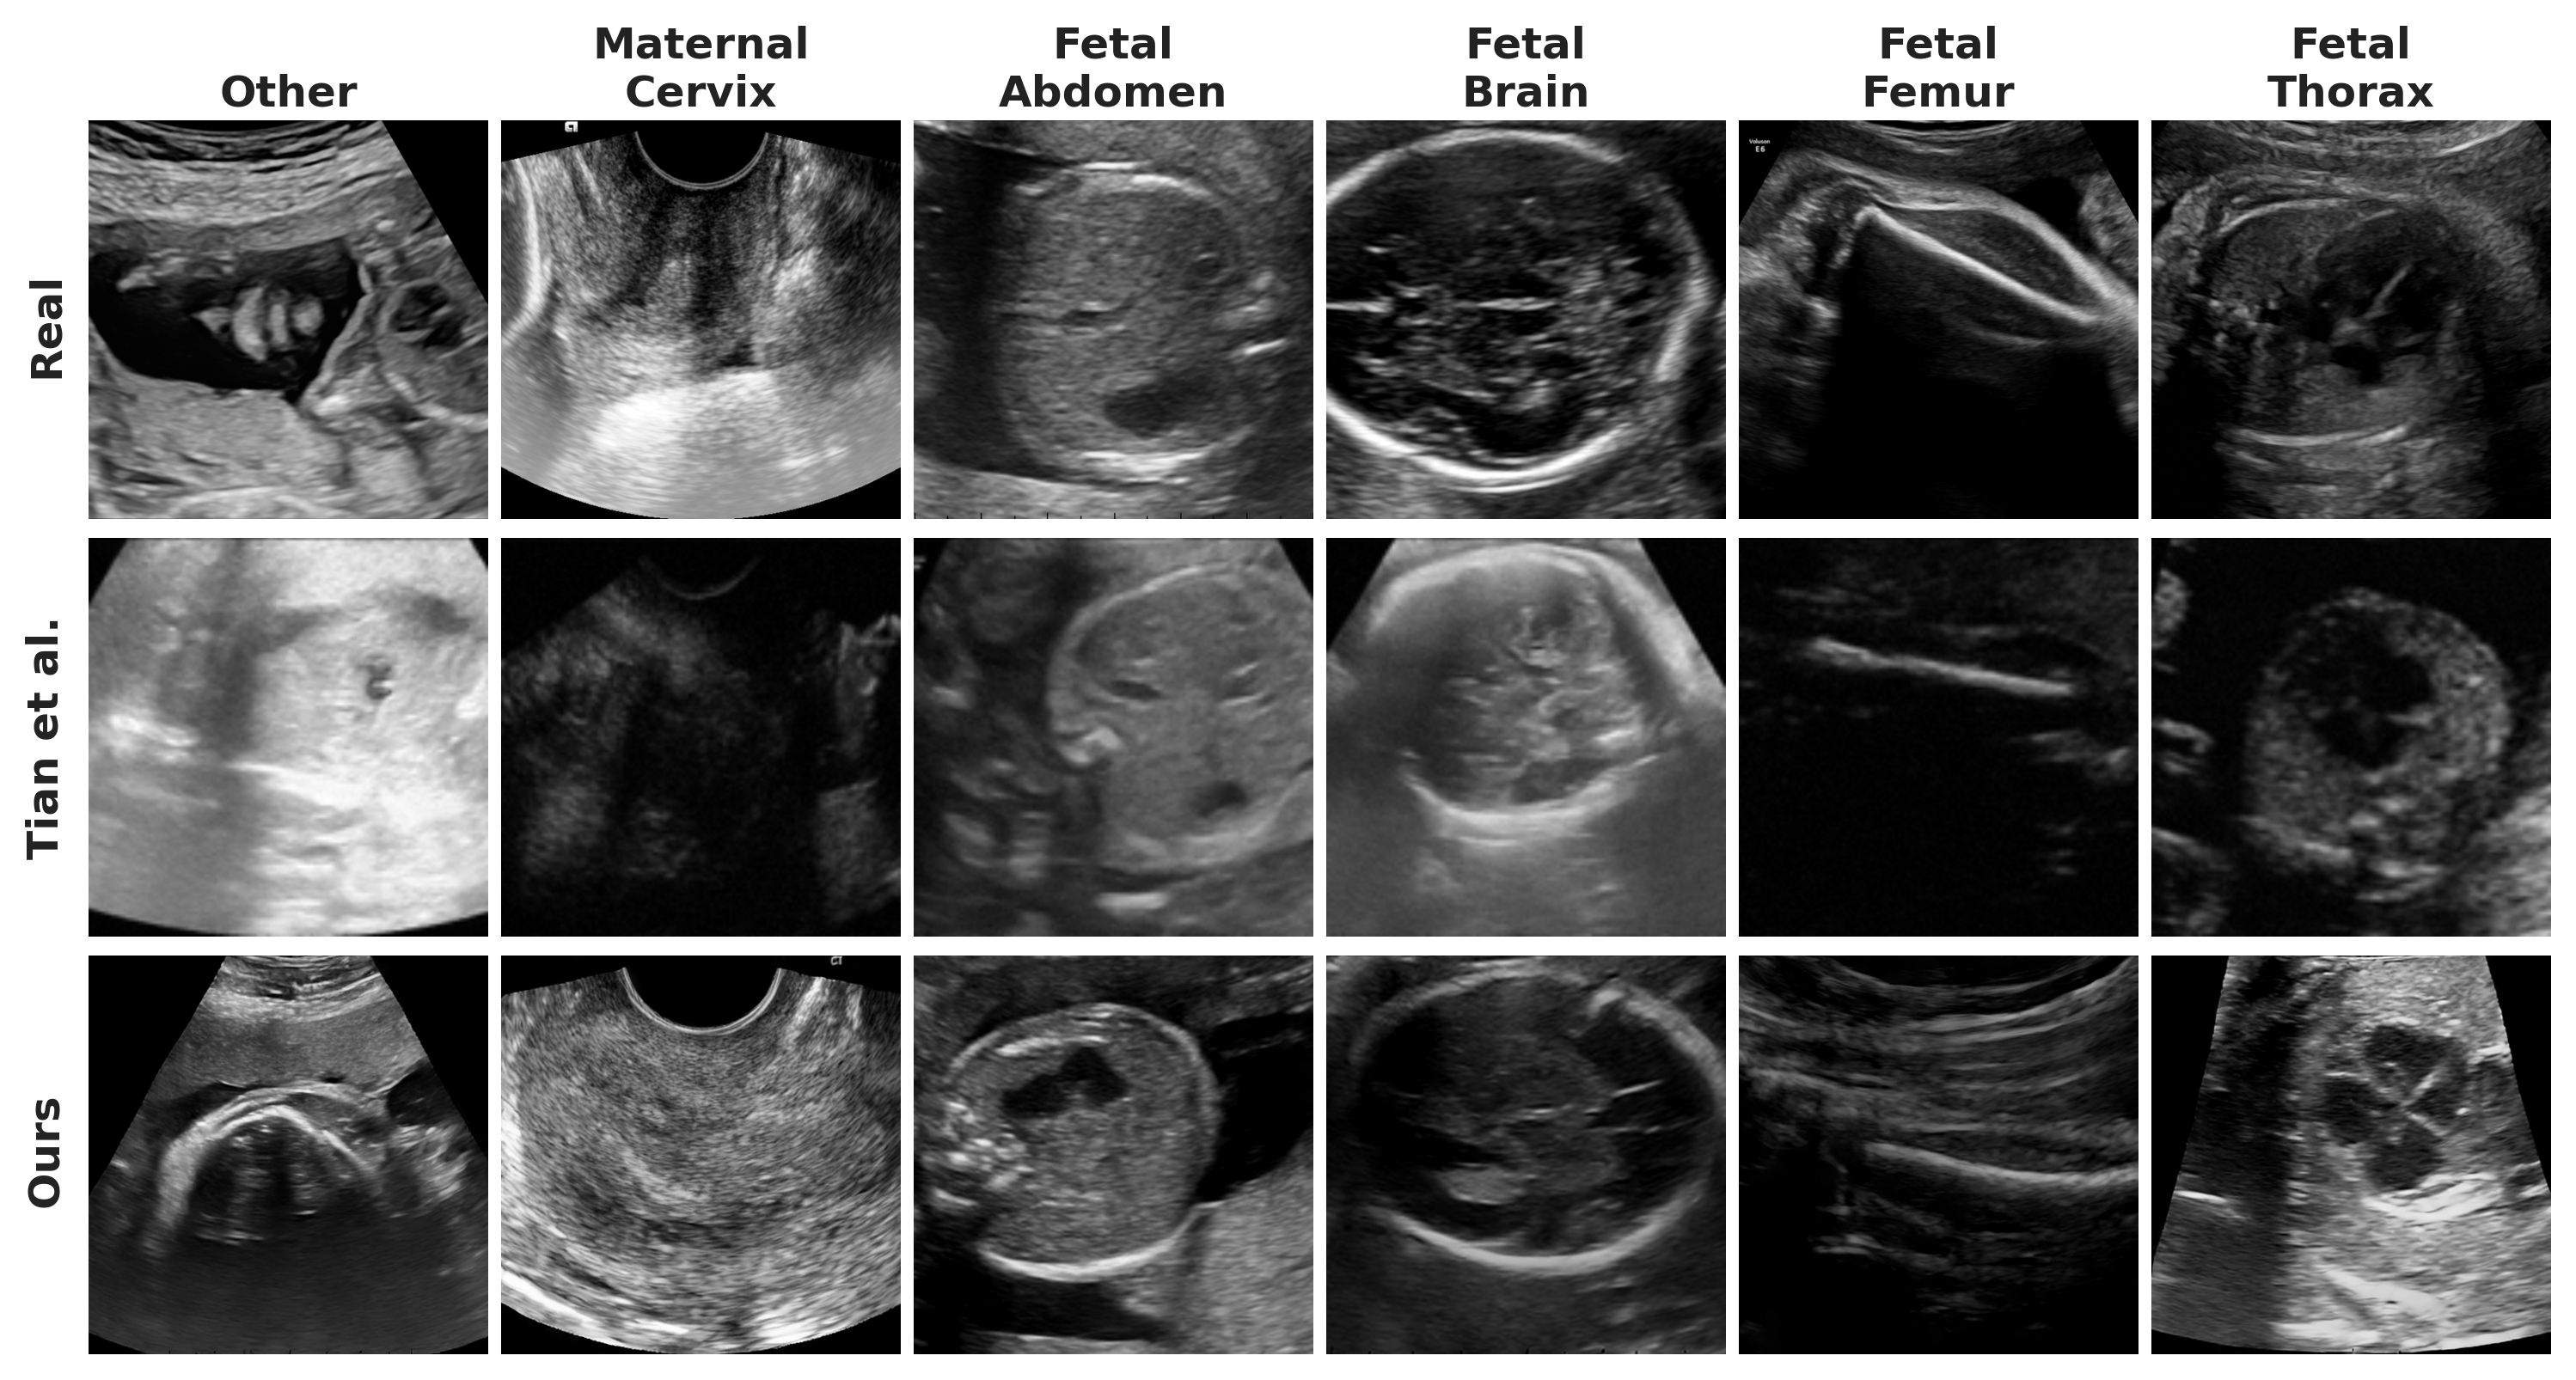
\includegraphics[width=0.4\linewidth]{image_grid.png}\label
  {fig:gen_images}

\vspace{-4mm}

\end{figure}

We evaluated the image quality of our image and compare them to \cite{tian2025enhancing} using Fréchet Inception Distance (FID) scores \cite{heusel2017gans}. We generate 5000 images for each of the six classes with a guidance scale of 2.25. For fair comparison, our images are downsized to 128 by 128. The results in Table \ref{tab:fid} show that our approach achieves higher quality in both individual classes and overall. Figure \ref{fig:gen_images} shows examples of generated images for each class.
Following Tian et al. \cite{tian2025enhancing}, who demonstrated that synthetic data improves fetal plane classification, we evaluated our high-resolution images using their top-performing architectures: ResNet50 \cite{he2016deep}, DenseNet169 \cite{huang2017densely}, and MedMamba \cite{yue2024medmamba}, plus a soft-voting ensemble. Using these specific models ensures a direct comparison with prior work.
%Tian et al. \cite{tian2025enhancing} showed that synthetic images could improve fetal plane classification performance. Building on this idea, we further evaluated the practical utility of our higher-resolution generated images through downstream fetal plane classification experiments using ResNet50, DenseNet169, and MedMamba, together with a soft-voting ensemble. These models were selected because they achieved the strongest classification performance in the evaluation reported by Tian et al., allowing a more direct comparison with prior work. 
We compared synthetic images generated by Tian et al. with our generated images under two settings: training from scratch on synthetic data only, and pretraining on synthetic data followed by real-world image fine-tuning. As shown in Table~\ref{tab:accuracy_comparison}, our images yielded stronger results when training from scratch, achieving 89.51\% ensemble accuracy. Under fine-tuning, our results also improved upon theirs, reaching a 93.36\% ensemble accuracy, surpassing the 92.32\% achieved on real-world data alone. These results suggest that our higher-resolution images are not only visually more realistic but also effective in supporting downstream classification performance.
%We compared synthetic images generated by Tian et al. with our generated images under two settings: training from scratch on synthetic data only, and pretraining on synthetic data followed by fine-tuning on real-world images. As shown in Table~\ref{tab:accuracy_comparison}, our generated images consistently yielded substantially stronger performance when training from scratch, achieving accuracies of 85.94\%, 87.67\%, and 86.34\% for ResNet50, DenseNet169, and MedMamba, respectively, with 89.51\% for the soft-voting ensemble, whereas classifiers trained on Tian et al.'s synthetic images performed poorly in this setting. Under fine-tuning, our results remained competitive and slightly improved over Tian et al. for most models, reaching 92.45\%, 92.15\%, and 91.77\%, with a soft-voting accuracy of 93.36\%. For reference, evaluation on the real-world FETAL\_PLANES\_DB dataset showed that the three individual models achieved accuracies above 90\%, while the ensemble reached 92.32\%. These results suggest that our higher-resolution synthetic images are not only visually more realistic, but also effective for supporting downstream classification with performance close to that obtained on real-world data.
%SURVEY
An experienced fetal ultrasound clinician (10 years’ expertise) evaluated 100 generated images, distinguishing real from synthetic and rating quality on a 5-point Likert scale. The mean score was 2.67, with real images scoring higher (3.12) than synthetic ones (2.07). Judgement relied on subtle artefacts including smoothing, speckle patterns, and anatomical inconsistencies.

\vspace{-5mm}
\begin{table}[htbp]
  \centering
  
  % --- First Table (Left) ---
  \begin{minipage}{0.4\textwidth}
    \centering
    \caption{FID comparison between Tian et al. \cite{tian2025enhancing} and our generated images.
    Lower FID indicates better image quality.}
    \label{tab:fid}
    \scriptsize
    \begin{tabular}{lcc}
      \toprule
      \bfseries Class & \bfseries Tian et al.  \cite{tian2025enhancing} & \bfseries Ours \\
      \midrule
      Other & 189.14 & \bf 143.30 \\
      Maternal cervix & 269.08 & \bf 155.30 \\
      Fetal abdomen & 241.14 & \bf 150.12 \\
      Fetal brain & 184.06 & \bf 117.71 \\
      Fetal femur & 203.10 & \bf 141.57 \\
      Fetal thorax & 233.37 & \bf 135.99 \\
      Overall & 176.85 & \bf 104.25 \\
      \bottomrule
    \end{tabular}
  \end{minipage}
  \hfill % Adds spacing between the two minipages
  % --- Second Table (Right) ---
  \begin{minipage}{0.56\textwidth}
    \centering
    \caption{Classifier accuracy comparison between Tian et al. \cite{tian2025enhancing} and our generated images.}
    \label{tab:accuracy_comparison}
    \scriptsize
    \begin{tabular}{llcc}
      \toprule
      \bfseries Method & \bfseries Model & \bfseries Tian et al. \cite{tian2025enhancing} & \bfseries Ours \\
      \midrule
      \multirow{4}{*}{\shortstack[l]{Training\\from\\Scratch}}
      & ResNet50     & 84.97\%  & \bf 85.94\% \\
      & DenseNet169  & 84.20\%  & \bf 87.67\% \\
      & MedMamba     & 82.53\%  & \bf 86.34\% \\
      & Soft Voting  & 87.35\%  & \bf 89.51\% \\
      \midrule
      \multirow{4}{*}{Fine-tuning}
      & ResNet50     & 91.29\% & \bf 92.45\% \\
      & DenseNet169  &  91.84\% & \bf 92.15\% \\
      & MedMamba     & 90.52\% & \bf 91.77\% \\
      & Soft Voting  & 92.84\% & \bf 93.36\% \\
      \bottomrule
    \end{tabular}
  \end{minipage}
\end{table}



\vspace{-12mm}
\section{Conclusions and future work}
We present an EDM2-based foundational model for high-resolution fetal ultrasound synthesis using open datasets, improving image quality and downstream classification performance. The model generates 512×512 images, surpassing prior 256×256 approaches. Clinical evaluation of 100 images yielded a mean score of 2.67/5, with real images rated higher than synthetic outputs. All code and models are released, with future work targeting scalable foundation models for low-resource healthcare and further comparison of diffusion architectures.

% \begin{credits}
% \subsubsection{\ackname} 
% This research was mainly supported by Studentship from the Faculty of Engineering and Physical Sciences - Electronic and Computer Science at the University of Southampton. The authors acknowledge the use of the IRIDIS X High Per- formance Computing Facility and the Southampton-Wolfson AI Research Machine (SWARM) GPU cluster, funded by the Wolfson Foundation, together with the associated support services at the University of Southampton in the completion of this work. The authors acknowledge the use of the UCL Unified AI Services Computing Facility (UAIServices@UCL), and associated support services, in the completion of this work.
% %%%%%%%%%%%%%%%%%%%%%%
% %UCL Unified AI
% % The authors acknowledge the use of the UCL Unified AI Services Computing Facility (UAIServices@UCL), and associated support services, in the completion of this work.


% \subsubsection{\discintname}
% The authors have no competing interests to declare that are relevant to the content of this article.
% % It is now necessary to declare any competing interests or to specifically
% % state that the authors have no competing interests. Please place the
% % statement with a bold run-in heading in small font size beneath the
% % (optional) acknowledgments\footnote{If EquinOCS, our proceedings submission
% % system, is used, then the disclaimer can be provided directly in the system.},
% % for example: The authors have no competing interests to declare that are
% % relevant to the content of this article. Or: Author A has received research
% % grants from Company W. Author B has received a speaker honorarium from
% % Company X and owns stock in Company Y. Author C is a member of committee Z.
% \end{credits}


%
% ---- Bibliography ----
%
% BibTeX users should specify bibliography style 'splncs04'.
% References will then be sorted and formatted in the correct style.
%
\bibliographystyle{splncs04}
%\bibliography{mybibliography}%%%OVERLEAF
\bibliography{../../latex/mybibliography}%%%GITHUB/ARXIV
% % This is samplepaper.tex, a sample chapter demonstrating the
% LLNCS macro package for Springer Computer Science proceedings;
% Version 2.21 of 2022/01/12
%


% Camera-ready submissions: All accepted papers must follow the below guidelines to submit your camera-ready papers –

% Your paper should contain your full authors names, full affiliation and ORCID ID (if available). Your submission should contain source files (e.g., latex files or word document). Please read the "Instructions for proceedings authors.pdf" carefully and make sure that you follow these instructions. The link is provided here: (opens in a new window)Instructions for proceedings authors.
% You should print, sign, and scan the "Licence to Publish Proceedings Papers". The license will be provided upon notification of acceptance. 
% Short papers: Authors are invited to submit short papers of length up to 3 pages excluding references (1 column – the LNCS template) showing proof-of-concept research contributions under the topics of the conference. All submissions will be peer-reviewed and the accepted abstracts will be published in Frontiers in Medical Technology as an ebook. Please use the template provided below.

% The word and character limits per short paper are as follows:
% -Title: 500 characters
% -Text: 1,000 words
% -Figures: 2
% -No Supplementary Material

% MIUA continues to foster fairness, diversity, and inclusion within its community. Submissions from typically underrepresented groups are particularly encouraged.

% https://www.ucd.ie/medicine/miua2026/calls/callforpapers/

% Reviewer #1
% Questions
% 1. Please provide major strengths of the paper.
% The paper presents a fetal ultrasound synthesis framework and shows that models trained on the proposed dataset achieve better performance than those trained on datasets used in previous work.

% 2. Please provide any major weaknesses of the paper.
% Although this is a short paper, the technical contribution appears weak. The proposed method is based on the existing EDM2 latent diffusion model, and the paper provides very limited implementation details, with no description of the training configuration beyond the loss function.


% 3. Overall evaluation of the paper.
% Accept


% 6. Constructive feedback to authors for improving the paper. (optional)
% It would be useful to include results from different network architectures trained on the same dataset with identical training configurations. The current version does not clearly demonstrate whether the observed performance is attributable to the EDM2 architecture or to the dataset used for training.

% KEY DATES
% Full Paper Submission: Thursday 2nd April 2026 (01:00 Pacific Time (PT))
% Notification of Acceptance: Friday 5th June 2026 
% Camera Ready Deadline: Friday 12th June 2026
% Early Registration: Friday 12th June 2026





\documentclass[runningheads]{llncs}
%
\usepackage[T1]{fontenc}
% T1 fonts will be used to generate the final print and online PDFs,
% so please use T1 fonts in your manuscript whenever possible.
% Other font encondings may result in incorrect characters.
%
\usepackage{booktabs} 
\usepackage{graphicx}
\usepackage{multirow}
\usepackage{orcidlink}
% Used for displaying a sample figure. If possible, figure files should
% be included in EPS format.
%
% If you use the hyperref package, please uncomment the following two lines
% to display URLs in blue roman font according to Springer's eBook style:
%\usepackage{color}
%\renewcommand\UrlFont{\color{blue}\rmfamily}
%\urlstyle{rm}

\vspace{-10mm}

\begin{document}
\title{
A Foundational EDM2-Based Generative Model for High-Resolution Synthetic Fetal Ultrasound Imaging from Open Datasets
}
%
%\titlerunning{Abbreviated paper title}
% If the paper title is too long for the running head, you can set
% an abbreviated paper title here
%

%\author{Anonymous Author(s)}

%\authorrunning{Anonymous Author(s)}
% First names are abbreviated in the running head.
% If there are more than two authors, 'et al.' is used.
%
%\institute{Affiliation(s)}

\author{Harvey Mannering\inst{1}\orcidlink{0000-0003-3094-7417} \and
Yilin Zhang\inst{1}\orcidlink{0009-0008-3660-5737}  \and
Ziao Liu\inst{2}\orcidlink{0009-0006-1905-1061} \and
Zhiwu Huang \inst{1}\orcidlink{0000-0002-7385-079X} \and
Jacqueline Matthew\inst{3}\orcidlink{0000-0003-4754-0322} \and
Miguel Xochicale\inst{4}\orcidlink{0000-0002-8225-7517}}


\authorrunning{H. Mannering et al.}
\titlerunning{EDM2-Based Fetal Ultrasound Generation}
% % First names are abbreviated in the running head.
% % If there are more than two authors, 'et al.' is used.
% %
\institute{
$^1$ University of Southampton,
$^2$ Tsinghua University,
$^3$ King's College London, \\
$^4$ University College London
\thanks{
Work on diffusion models with the U. of Southampton supported by PhD studentship, Tsinghua University (classification), KCL (clinical evaluation) and reproducible workflows and robust software engineering on UCL-ARC’s Unified-AI cloud platform.
}
}


\maketitle              % typeset the header of the contribution

\vspace{-5mm}
% The abstract should briefly summarize the contents of the paper in 150--250 words.
\begin{abstract}
Prenatal ultrasound imaging is key for assessing fetal health, but AI progress is limited by scarce, privacy-restricted, and hard-to-annotate datasets. 
We propose a high-resolution fetal ultrasound synthesis framework based on the EDM2 diffusion architecture, trained on multiple public datasets to generate 512×512 images across six anatomical classes. Our method achieved improved image quality with lower FID scores and enhanced downstream fetal plane classification, reaching 93.36\% ensemble accuracy after fine-tuning, surpassing real-data-only training. 
Clinical evaluation by an experienced fetal ultrasound specialist (10+ years) on 100 images yielded a mean realism score of 2.67/5, with real images rated higher than synthetic. Artefacts included smoothing, speckle irregularities, and anatomical inconsistencies. 
Code, data, models and other resources to reproduce this work are available at \url{https://github.com/xfetus/fetal-ultrasound-edm2}.
\keywords{
Fetal Ultrasound \and 
% Diffusion Models \and 
Synthetic Medical Imaging
}
\end{abstract}


\vspace{-9mm}
\section{Introduction}
Prenatal ultrasound (US) imaging is the primary modality for assessing fetal health and development. Recent advances in AI have accelerated the development of classifiers, automated detection systems, and synthetic image generation methods for prenatal imaging. However, clinically reliable AI models require diverse datasets that capture real-world complexity, including varied fetal conditions, US scanners, patient demographics, and imaging modalities from 2D to emerging 3D-4D US \cite{kurjak2007useful}. Additional challenges include inconsistent volumetric assessment protocols, operator-dependent variability between sonographers, and natural anatomical variation between patients and fetuses \cite{jcm13185626}. 
Open datasets and evaluation frameworks are therefore essential for assessing AI model fidelity, robustness, and diversity \cite{IBRAHIM2025}.
Recently, \cite{Alsharid2025} published a comprehensive overview of publicly available US resources, including datasets and deep learning models, which is highly relevant to open-source strategies in US imaging. 
However, fetal US datasets remain largely centred on the FETAL PLANES DB, which contains 12,400 images \cite{burgos2020evaluation}. \cite{Alsharid2025} also reports additional emerging datasets, including the US Fetus Phantom dataset (15,728 images), the Fetal Head dataset (1,334 images), the Fetal Abdomen dataset (4,668 images), and the Fetal Cardiac dataset (300 images).
Parallel to this work, generative models such as GANs \cite{Goodfellow2014}, VAE \cite{kingma2013auto}, diffusion models \cite{ho2020_neurips}, and flow-based models \cite{lipman2022flow} are now a promising avenue to address data scarcity in medical images \cite{yan2018generation,tian2025enhancing}.
Diffusion-Based Fetal US Synthesis with Active Learning presented promising results on image quality comparison with baseline models but no clinical evaluation is included \cite{Arjemandi2026}. In US images, Stable Diffusion 1.5 \cite{rombach2022high} with ControlNet \cite{zhang2023adding} has enabled localized tumor synthesis \cite{freiche2025ultrasound}, while Tian et al. \cite{tian2025enhancing} utilized diffusion-generated images to improve plane classification, although only at $128 \times 128$ resolution. While hybrid Diffusion-GAN approaches \cite{iskandar2023towards} reached $256 \times 256$, these resolutions remain clinically restrictive and rely on older architectures. By contrast, we apply EDM2 \cite{karras2024analyzing}, the current state of the art for ImageNet generation \cite{deng2009imagenet}, to synthesize high-fidelity fetal US images at a more realistic $512 \times 512$ resolution.

%%%%%%%%%%%%%%%%%%%%%%%%%%%%%%%%%%%%%%%%%%%%%%%%%%%%%%%%%%%%%%%%%%%%%%%%%%%%%
%%%%%%%%%%%%%%%%%%%%%%%%%%%%%%%%%%%%%%%%%%%%%%%%%%%%%%%%%%%%%%%%%%%%%%%%%%%%%
%%%%%%%%%%%%%%%%%%%%%%%%%%%%%%%%%%%%%%%%%%%%%%%%%%%%%%%%%%%%%%%%%%%%%%%%%%%%%
\section{Methods and datasets}

We trained the EDM2 diffusion model to generate 6 US images classes with center cropping, random horizontal flipping, and resizing to $512 \times 512$, following the training setup from \cite{tian2025enhancing}, except with a higher resolution. We train two different sized networks, EDM2-S and EDM2-XL, which allows us to apply autoguidance \cite{karras2024guiding} to improve image quality.
We focus on the FETAL PLANES DB dataset (12,400 images) \cite{burgos2020evaluation}, which includes six classes: maternal cervix, fetal abdomen, fetal brain, fetal femur, fetal thorax, and other.
However, this dataset is relatively small, there is a risk of the diffusion model memorizing training data.
To mitigate this, we incorporate additional datasets: the FPU23 dataset (15,728 images) \cite{prabakaran2023fpus23}, a fetal abdominal structures segmentation dataset (1,588 images) \cite{da2023fetal}, and an African low-resource dataset (451 images) \cite{sendra2023generalisability}.
Each additional dataset is given a single label during training. 
We use a weighted MSE loss, weighting FETAL PLANES DB at 2.0 and others at 1.0.
Including these datasets allows twice as many training steps and reduces validation loss from 0.1427 to 0.1371.

\section{Experiments and results}

\begin{figure}[htbp]
\centering
  \caption{
  Representative fetal ultrasound images from real data, Tian et al. \cite{tian2025enhancing}, and our proposed high-resolution ($512 \times 512$) diffusion-based synthesis approach.
  Higher resolution image at our repository  \url{https://github.com/xfetus/fetal-ultrasound-edm2}.
  }
  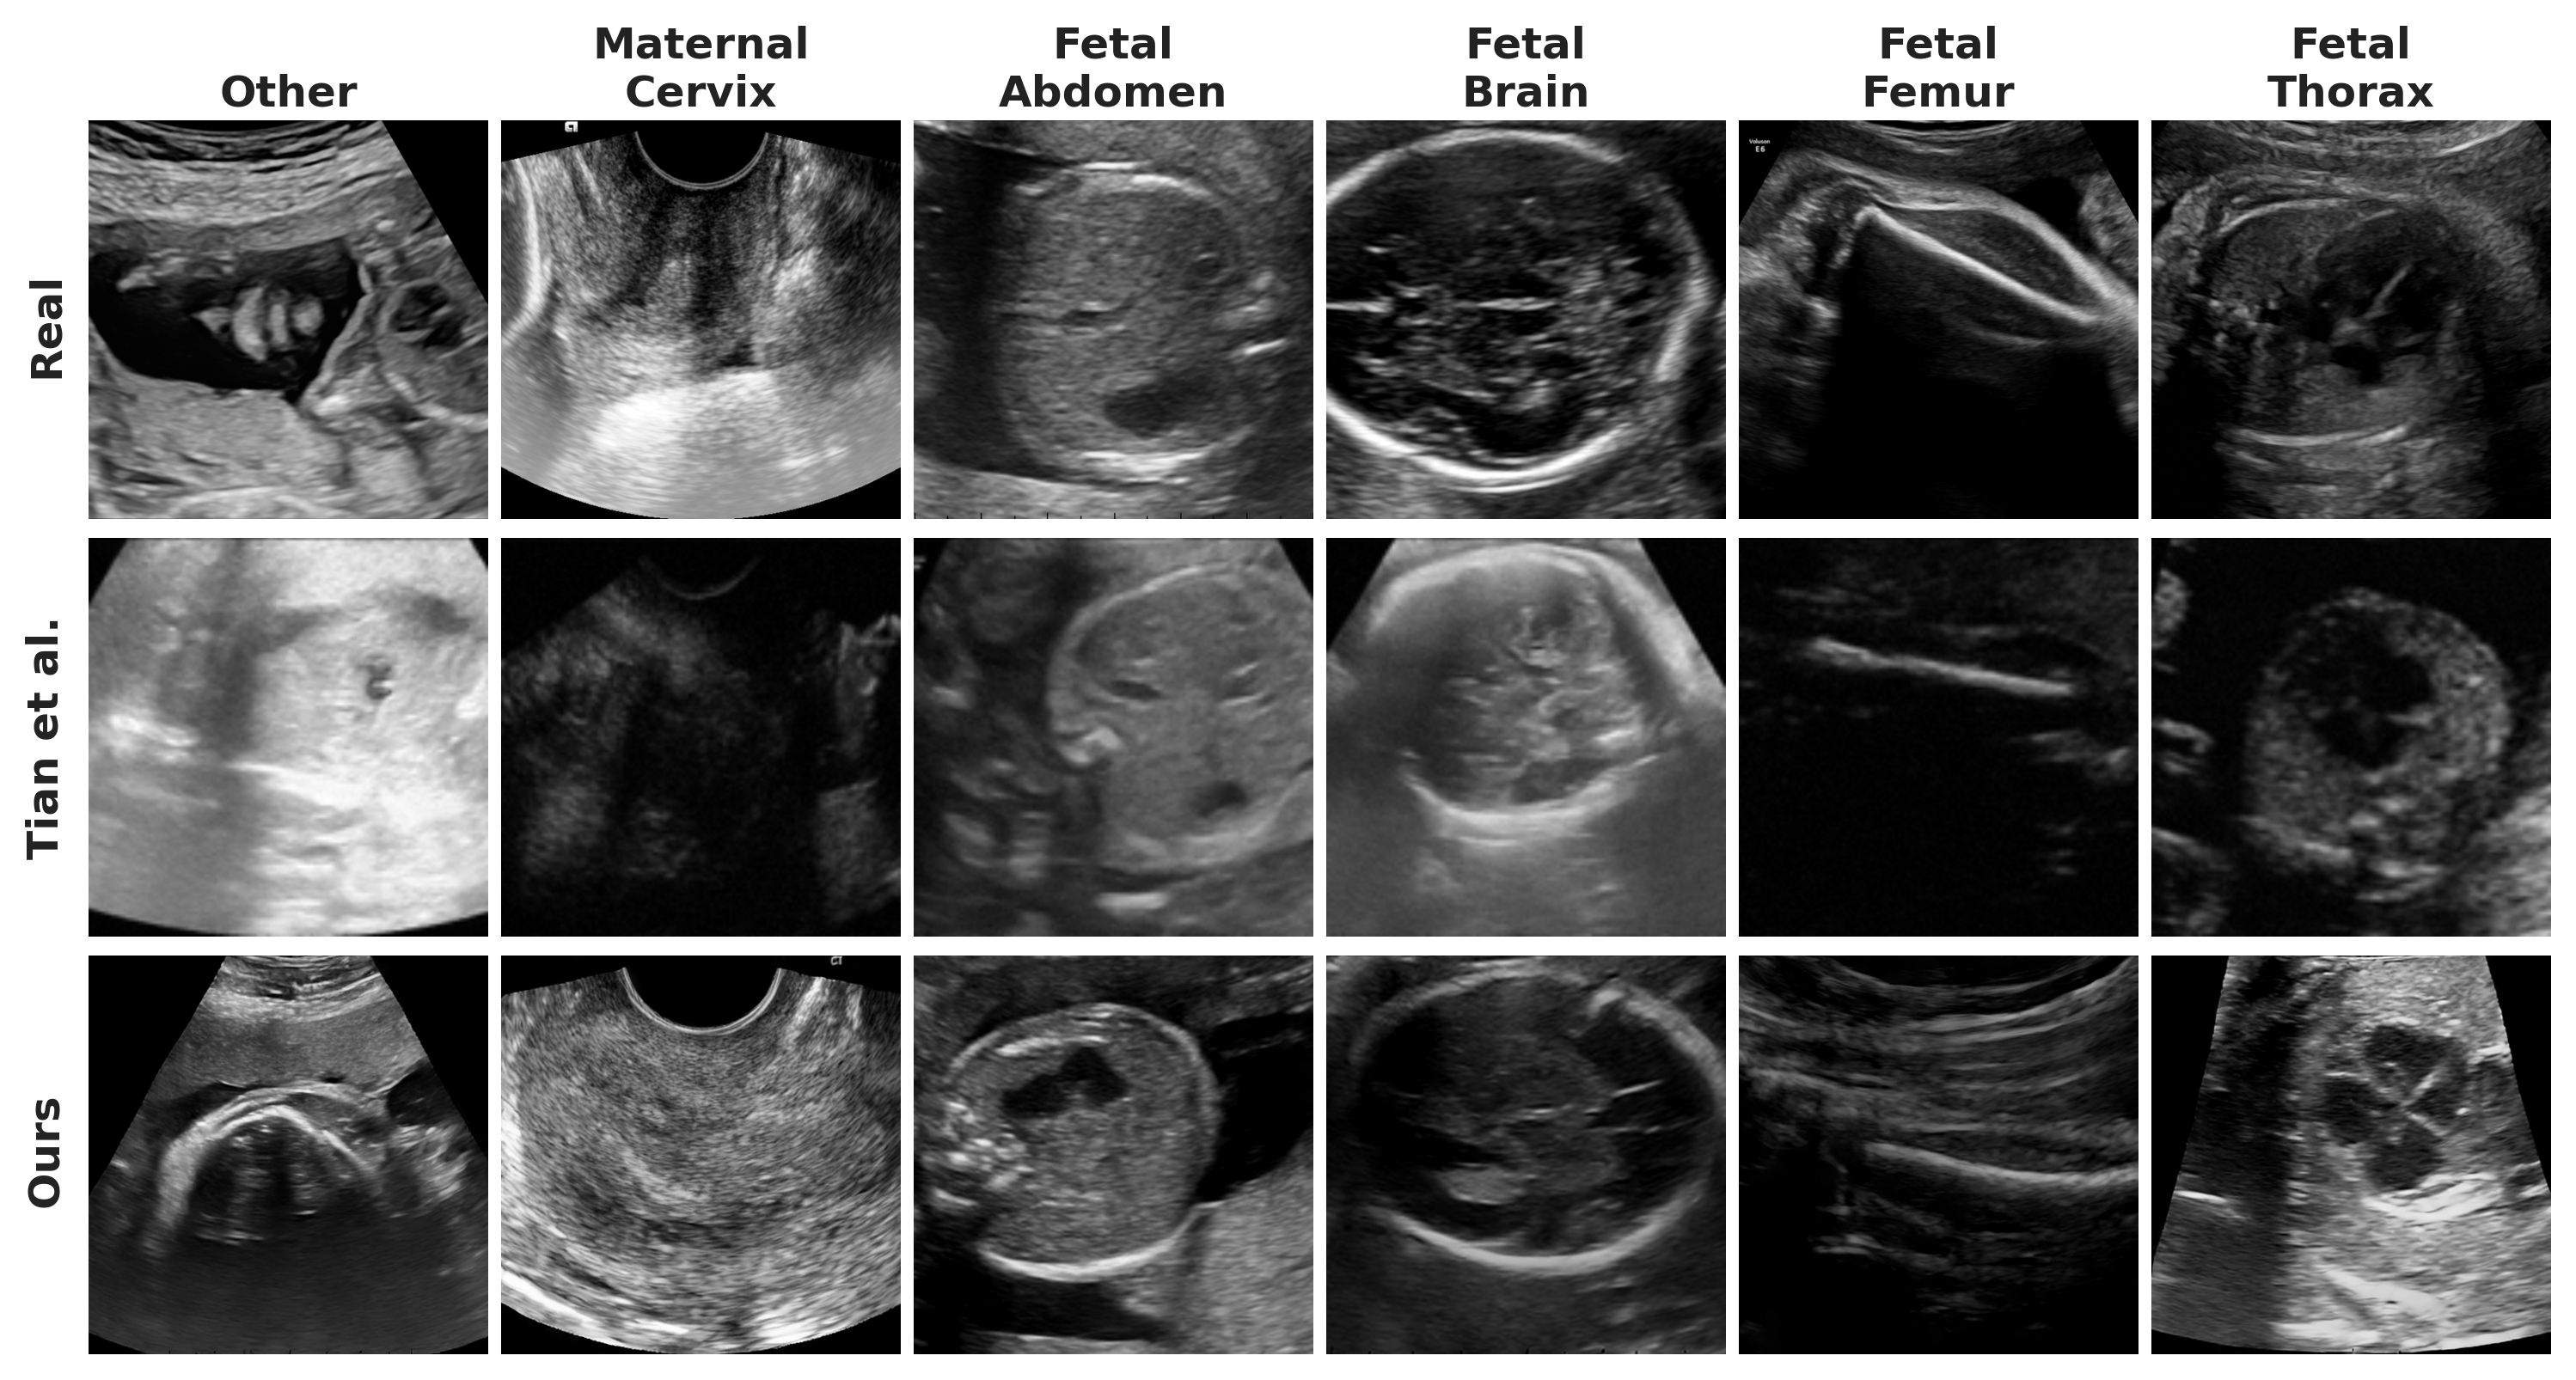
\includegraphics[width=0.4\linewidth]{image_grid.png}\label
  {fig:gen_images}

\vspace{-4mm}

\end{figure}

We evaluated the image quality of our image and compare them to \cite{tian2025enhancing} using Fréchet Inception Distance (FID) scores \cite{heusel2017gans}. We generate 5000 images for each of the six classes with a guidance scale of 2.25. For fair comparison, our images are downsized to 128 by 128. The results in Table \ref{tab:fid} show that our approach achieves higher quality in both individual classes and overall. Figure \ref{fig:gen_images} shows examples of generated images for each class.
Following Tian et al. \cite{tian2025enhancing}, who demonstrated that synthetic data improves fetal plane classification, we evaluated our high-resolution images using their top-performing architectures: ResNet50 \cite{he2016deep}, DenseNet169 \cite{huang2017densely}, and MedMamba \cite{yue2024medmamba}, plus a soft-voting ensemble. Using these specific models ensures a direct comparison with prior work.
%Tian et al. \cite{tian2025enhancing} showed that synthetic images could improve fetal plane classification performance. Building on this idea, we further evaluated the practical utility of our higher-resolution generated images through downstream fetal plane classification experiments using ResNet50, DenseNet169, and MedMamba, together with a soft-voting ensemble. These models were selected because they achieved the strongest classification performance in the evaluation reported by Tian et al., allowing a more direct comparison with prior work. 
We compared synthetic images generated by Tian et al. with our generated images under two settings: training from scratch on synthetic data only, and pretraining on synthetic data followed by real-world image fine-tuning. As shown in Table~\ref{tab:accuracy_comparison}, our images yielded stronger results when training from scratch, achieving 89.51\% ensemble accuracy. Under fine-tuning, our results also improved upon theirs, reaching a 93.36\% ensemble accuracy, surpassing the 92.32\% achieved on real-world data alone. These results suggest that our higher-resolution images are not only visually more realistic but also effective in supporting downstream classification performance.
%We compared synthetic images generated by Tian et al. with our generated images under two settings: training from scratch on synthetic data only, and pretraining on synthetic data followed by fine-tuning on real-world images. As shown in Table~\ref{tab:accuracy_comparison}, our generated images consistently yielded substantially stronger performance when training from scratch, achieving accuracies of 85.94\%, 87.67\%, and 86.34\% for ResNet50, DenseNet169, and MedMamba, respectively, with 89.51\% for the soft-voting ensemble, whereas classifiers trained on Tian et al.'s synthetic images performed poorly in this setting. Under fine-tuning, our results remained competitive and slightly improved over Tian et al. for most models, reaching 92.45\%, 92.15\%, and 91.77\%, with a soft-voting accuracy of 93.36\%. For reference, evaluation on the real-world FETAL\_PLANES\_DB dataset showed that the three individual models achieved accuracies above 90\%, while the ensemble reached 92.32\%. These results suggest that our higher-resolution synthetic images are not only visually more realistic, but also effective for supporting downstream classification with performance close to that obtained on real-world data.
%SURVEY
An experienced fetal ultrasound clinician (10 years’ expertise) evaluated 100 generated images, distinguishing real from synthetic and rating quality on a 5-point Likert scale. The mean score was 2.67, with real images scoring higher (3.12) than synthetic ones (2.07). Judgement relied on subtle artefacts including smoothing, speckle patterns, and anatomical inconsistencies.

\vspace{-5mm}
\begin{table}[htbp]
  \centering
  
  % --- First Table (Left) ---
  \begin{minipage}{0.4\textwidth}
    \centering
    \caption{FID comparison between Tian et al. \cite{tian2025enhancing} and our generated images.
    Lower FID indicates better image quality.}
    \label{tab:fid}
    \scriptsize
    \begin{tabular}{lcc}
      \toprule
      \bfseries Class & \bfseries Tian et al.  \cite{tian2025enhancing} & \bfseries Ours \\
      \midrule
      Other & 189.14 & \bf 143.30 \\
      Maternal cervix & 269.08 & \bf 155.30 \\
      Fetal abdomen & 241.14 & \bf 150.12 \\
      Fetal brain & 184.06 & \bf 117.71 \\
      Fetal femur & 203.10 & \bf 141.57 \\
      Fetal thorax & 233.37 & \bf 135.99 \\
      Overall & 176.85 & \bf 104.25 \\
      \bottomrule
    \end{tabular}
  \end{minipage}
  \hfill % Adds spacing between the two minipages
  % --- Second Table (Right) ---
  \begin{minipage}{0.56\textwidth}
    \centering
    \caption{Classifier accuracy comparison between Tian et al. \cite{tian2025enhancing} and our generated images.}
    \label{tab:accuracy_comparison}
    \scriptsize
    \begin{tabular}{llcc}
      \toprule
      \bfseries Method & \bfseries Model & \bfseries Tian et al. \cite{tian2025enhancing} & \bfseries Ours \\
      \midrule
      \multirow{4}{*}{\shortstack[l]{Training\\from\\Scratch}}
      & ResNet50     & 84.97\%  & \bf 85.94\% \\
      & DenseNet169  & 84.20\%  & \bf 87.67\% \\
      & MedMamba     & 82.53\%  & \bf 86.34\% \\
      & Soft Voting  & 87.35\%  & \bf 89.51\% \\
      \midrule
      \multirow{4}{*}{Fine-tuning}
      & ResNet50     & 91.29\% & \bf 92.45\% \\
      & DenseNet169  &  91.84\% & \bf 92.15\% \\
      & MedMamba     & 90.52\% & \bf 91.77\% \\
      & Soft Voting  & 92.84\% & \bf 93.36\% \\
      \bottomrule
    \end{tabular}
  \end{minipage}
\end{table}



\vspace{-12mm}
\section{Conclusions and future work}
We present an EDM2-based foundational model for high-resolution fetal ultrasound synthesis using open datasets, improving image quality and downstream classification performance. The model generates 512×512 images, surpassing prior 256×256 approaches. Clinical evaluation of 100 images yielded a mean score of 2.67/5, with real images rated higher than synthetic outputs. All code and models are released, with future work targeting scalable foundation models for low-resource healthcare and further comparison of diffusion architectures.

% \begin{credits}
% \subsubsection{\ackname} 
% This research was mainly supported by Studentship from the Faculty of Engineering and Physical Sciences - Electronic and Computer Science at the University of Southampton. The authors acknowledge the use of the IRIDIS X High Per- formance Computing Facility and the Southampton-Wolfson AI Research Machine (SWARM) GPU cluster, funded by the Wolfson Foundation, together with the associated support services at the University of Southampton in the completion of this work. The authors acknowledge the use of the UCL Unified AI Services Computing Facility (UAIServices@UCL), and associated support services, in the completion of this work.
% %%%%%%%%%%%%%%%%%%%%%%
% %UCL Unified AI
% % The authors acknowledge the use of the UCL Unified AI Services Computing Facility (UAIServices@UCL), and associated support services, in the completion of this work.


% \subsubsection{\discintname}
% The authors have no competing interests to declare that are relevant to the content of this article.
% % It is now necessary to declare any competing interests or to specifically
% % state that the authors have no competing interests. Please place the
% % statement with a bold run-in heading in small font size beneath the
% % (optional) acknowledgments\footnote{If EquinOCS, our proceedings submission
% % system, is used, then the disclaimer can be provided directly in the system.},
% % for example: The authors have no competing interests to declare that are
% % relevant to the content of this article. Or: Author A has received research
% % grants from Company W. Author B has received a speaker honorarium from
% % Company X and owns stock in Company Y. Author C is a member of committee Z.
% \end{credits}


%
% ---- Bibliography ----
%
% BibTeX users should specify bibliography style 'splncs04'.
% References will then be sorted and formatted in the correct style.
%
\bibliographystyle{splncs04}
%\bibliography{mybibliography}%%%OVERLEAF
\bibliography{../../latex/mybibliography}%%%GITHUB/ARXIV
% \input{main.bbl}%%%ARXIV

\end{document}
%%%ARXIV

\end{document}
%%%ARXIV

\end{document}
%%%ARXIV

\end{document}
